% File project.tex
%% Style files for ACL 2021
\documentclass[11pt,a4paper]{article}
\usepackage[hyperref]{acl2021}
\usepackage{times}
\usepackage{booktabs}
\usepackage{todonotes}
\usepackage{latexsym}
\usepackage{amsfonts}
\usepackage{graphicx}
\usepackage{amsmath}
\usepackage{multirow} 
\usepackage{xcolor}
\usepackage{subfigure}
\usepackage{subcaption}
\usepackage{hyperref}

\renewcommand{\UrlFont}{\ttfamily\small}

% This is not strictly necessary, and may be commented out,
% but it will improve the layout of the manuscript,
% and will typically save some space.
\usepackage{microtype}

\aclfinalcopy 

\newcommand\BibTeX{B\textsc{ib}\TeX}

\title{VOLNet: An Aligned Approach for Visual-LiDAR Odometry}

\author{
  Ming-Feng Li\thanks{\hspace{4pt}Everyone Contributed Equally -- Alphabetical order} \hspace{2em} Pujith Kachana$^*$ \hspace{2em} Shashwat Chawla$^*$ \hspace{2em} Yatharth Ahuja $^*$ \\
  \texttt{\{mingfenl, pkachana, shashwac, yahuja\}@andrew.cmu.edu}
  }


\date{}

\begin{document}
\maketitle
\begin{abstract}
Visual Odometry (VO), or the estimation of camera motions from sequential RGB frames, is essential in autonomous systems and visual SLAM. Traditional geometry-based methods often face challenges in environments with dynamic obstacles and rapid movements. To enhance performance, learning-based monocular VO approaches like TartanVO have been developed, demonstrating significant real-world effectiveness. However, these methods struggle with scale ambiguity due to a lack of inherent depth information. To address this, we propose \textbf{VOLNet}, a Visual-LiDAR Odometry method that integrates RGB images with LiDAR data with explicit alignment, harnessing the semantic richness of RGB images and the precise geometric details from 3D LiDAR point clouds. This multimodal approach underscores the potential for improved odometry tasks. Typically trained on limited datasets such as KITTI, existing methods do not adequately adapt to varied and dynamic real-world scenarios. We train on TartanAir-v2, a large-scale synthetic dataset that includes diverse indoor and outdoor environments. Our method, free from time-sync and camera calibration issues, leverages high-quality synthetic data to demonstrate enhanced estimation accuracy and superior cross-dataset generalizability, pushing the boundaries of existing Visual-LiDAR Odometry baselines.

\end{abstract}

\section{Introduction and Problem Definition}
Accurate 3D localization is fundamental for autonomous systems, facilitating precise movement tracking in autonomous vehicles, robots, and drones. Visual odometry (VO), crucial for estimating camera motions from sequential RGB frames, plays an essential role in integrating RGB information with LiDAR sensors for various navigation and mapping tasks. For instance, Visual Simultaneous Localization and Mapping (SLAM) is increasingly vital due to the widespread availability of cameras and relies heavily on visual odometry.
Traditional geometry-based methods are foundational but often struggle in complex environments with dynamic obstacles and rapid movements. In contrast, recent learning-based methods, while promising, lack the intrinsic geometric grounding of traditional approaches.
Current visual odometry predominantly employs monocular camera systems, which, although cost-effective and broadly applicable, are limited by their inability to reliably determine depth, leading to potential inaccuracies in scale and overall pose estimation. These systems also typically underperform in challenging environmental conditions, such as poor lighting or the presence of dynamic objects, which can disrupt feature tracking continuity and reliability.

Moreover, most existing VO methods are trained and validated on relatively constrained datasets like KITTI, which primarily feature well-controlled urban driving scenarios. These datasets fail to capture the complexity and diversity of real-world environments, thus limiting the generalizability of these methods to scenarios beyond typical urban conditions, such as off-road environments or areas with highly dynamic and unpredictable elements.

To overcome these challenges, we propose leveraging the large-scale synthetic dataset, TartanAir-v2, which features a variety of environments and realistic instances, to address the limitations of limited real-world training data. Additionally, we propose a hybrid Visual-LiDAR Odometry system that integrates the semantic richness of RGB images with the geometric precision of 3D LiDAR point clouds. Our approach involves estimating the optical flow map between two neighboring images to ascertain their semantic correspondences. Concurrently, we project LiDAR points into 2D depth maps aligned with the RGB images. The RGB images, flow maps, and projected depth maps of LiDAR points are then concatenated and fed into a transformer-based network to estimate the final relative camera pose between the images.

By benefiting from the synthetic dataset, our approach not only improves the reliability of localization under various operational conditions but also extends the applicability of VO systems to more dynamic and unstructured environments. Leveraging high-quality images and accurate LiDAR data, our system demonstrates the complementary strengths of each sensor type, enhancing the robustness and accuracy of odometry across diverse environments.




\subsection{Problem Definition.} For visual-LiDAR odometry, we are provided with a sequence of $n$ RGB test images, $\mathcal{I} = \{I_0, I_1, \dots, I_{n-1}\}$, and corresponding LiDAR point clouds $\mathcal{L} = \{L_0, L_1, \dots, L_{n-1}\}$. Our method aims to estimate the relative camera pose ${\xi}i$ for each pair of consecutive test images $(I_i, I{i+1})$ and their respective LiDAR scans $(L_i, L_{i+1})$. Each estimation ${\xi}i$ is represented as a rotation quaternion $q \in \mathbb{R}^4$ and a translation vector $t \in \mathbb{R}^3$, which describe the orientation and position changes between two consecutive frames. For each estimation, we fuse the inputs from $(I_i, I{i+1})$ and $(L_i, L_{i+1})$, and then send them to a trained model that predicts ${\xi}_i$. This process leverages both visual and geometric data to enhance accuracy in pose estimation.

\subsection{Contributions}

Our proposed solution involves training a visual-LiDAR odometry model on the TartanAir-v2 dataset, a comprehensive synthetic dataset designed to simulate a wide range of environmental conditions. This training approach aims to overcome the limitations of existing models by including scenes with significant environmental variability and dynamic obstacles, thereby ensuring that our models are better prepared for real-world deployment. We contribute a novel learning-based visual-LiDAR model \textbf{VOLNet} with explicit alignment between the RBG and LiDAR data that is robust to camera parameters, understands scale, and is data-driven and scalable.  Through this approach, we seek to set new benchmarks in estimation accuracy and adaptability for Visual-LiDAR Odometry systems, pushing the boundaries of what is currently achievable in autonomous navigation.


\clearpage
\section{Related Work and Background}

Odometry serves as a fundamental component in robotic navigation, facilitating accurate estimation of a robot’s position and motion over time. It has been an active research avenue with various landmark works over time - 
Mur-Artal et al. proposed ORB-SLAM \cite{orb-slam}, a real-time monocular visual SLAM framework leveraging ORB features for robust odometry and loop closure detection, demonstrating state-of-the-art accuracy in both indoor and outdoor environments. Zhang and Scaramuzza introduced VIO (Visual-Inertial Odometry) \cite{vio}, combining visual and inertial measurements to address challenges posed by low-texture and dynamic lighting conditions, enabling robust navigation across diverse scenarios. Similarly, Lego-LOAM \cite{legoloam} advanced LiDAR odometry by incorporating both edge and surface features to enhance accuracy and robustness in complex 3D environments. For multi-modal systems, Kimera (Rosinol et al., 2020) integrated visual, inertial, and geometric data to achieve metric-semantic SLAM, enhancing odometry performance in dynamic and cluttered spaces. Further, Wang et al. employed deep learning in DeepVO \cite{deepVO} to learn odometry directly from sequential image data, showcasing the potential of data-driven methods for end-to-end trajectory estimation. These works collectively underscore the evolution of odometry from classical feature-based approaches to modern multi-modal and learning-based paradigms, addressing the increasing demands of autonomous systems. We explore the odometry estimation landscape in a more classified manner in this section.

\subsection{Related Datasets} 
\noindent \textbf{KITTI Odometry.}
The KITTI odometry dataset \cite{KITTI} is a widely used benchmark for evaluating odometry and SLAM systems. This dataset includes 22 sequences of LiDAR point clouds and corresponding stereo images. For the purposes of this study, we utilize only the monocular left camera images for fusion with the LiDAR sensor.

\noindent \textbf{TartanAir.}
The TartanAir dataset \cite{tartanair} is a large-scale, synthetically generated vision and navigation dataset rendered using the Unreal Engine. The synthetic nature of the data guarantees precise, dense measurements, while the well-developed rendering process keeps the data reasonably photo-realistic.

\noindent \textbf{TartanAir-v2.}
Building on the foundation of TartanAir, the TartanAir-v2 dataset expands the scale and richness of the data significantly. TartanAir-v2 introduces 100 unique environments, each featuring more sequences and an even greater variety of data modalities. Most notably, TartanAir-v2 includes a LiDAR modality which we make use of for this project.

\subsection{Traditional Visual Odometry}

For the RGB modality, the classical unimodal baseline \textbf{ORB-SLAM} \cite{orb-slam} extracts ORB features from images and uses them to establish correspondences between consecutive frames. By applying epipolar constraints and classical optimization techniques, it estimates camera poses, which are further refined through global optimization using a pose graph and loop closure. ORB-SLAM will establish a baseline for the accuracy achievable with monocular RGB images and geometric analysis, supporting our hypothesis that RGB images provide strong visual features for odometry.

\subsection{Traditional LiDAR Odometry}
For the LiDAR modality, the unimodal classical baseline \textbf{ICP-SLAM} \cite{KISS-ICP} leverages ICP (Iterative Closest Points) to compute correspondences between two point sets by identifying the nearest neighbors and then calculating the transformation that minimizes the distance between these approximated correspondences. This process is repeated until the transformation converges below a threshold or reaches a maximum number of iterations. ICP can be effective with consecutive frames, although its accuracy diminishes in the presence of noise or lower sampling rates. This method will serve as a baseline to gauge the accuracy achievable with LiDAR alone and assess how well LiDAR’s inherent 3D structure can be utilized.

\subsection{Traditional Visual-LiDAR Odometry}
To enhance the accuracy and robustness of odometry and mapping tasks, advanced baselines such as \textbf{DV-LOAM} \cite{dv-loam} and \textbf{SDV-LOAM} \cite{sdv-loam} effectively integrate visual and LiDAR information. \textbf{DV-LOAM} utilizes frame-to-frame tracking and sliding window optimization for efficient pose estimation, refining keyframe poses with LiDAR data, which is particularly beneficial in environments with sparse visual features. Extending these capabilities, \textbf{SDV-LOAM} incorporates semi-direct approaches like LiDAR-Assisted Visual Odometry to improve depth estimation and adapt to dynamic environments. Its cascaded Vision-LiDAR architecture harmonizes direct visual odometry with precise LiDAR measurements for more accurate and robust pose estimates. Traditional methods, such as \textbf{V-LOAM} \cite{zhang2015visual} and \textbf{LIMO} \cite{graeter2018limo}, also leverage high-frequency visual odometry estimates as motion priors for LiDAR, with \textbf{LIMO} utilizing depth information to mitigate scale uncertainty. Additionally, \textbf{PL-LOAM} \cite{huang2020lidar} provides novel scale correction algorithms alongside pure visual tracking methods, further bridging the gap between 3D and 2D data integration challenges.

% \subsection{Deep Visual Odometry}

% Recent advancements in learning-based methods have significantly enhanced the capabilities of visual odometry systems. The pioneering work~\cite{konda2015learning} utilized deep neural networks to estimate odometry by predicting both the speed and direction from individual images. Following this, methods such as those introduced in~\cite{kendall2015posenet} utilized Convolutional Neural Networks (CNNs) to extract features from images for pose estimation. Further advancements include DeepVO~\cite{wang2017deepvo}, which applied deep recurrent neural networks to capture the temporal dynamics and dependencies of sequences, thereby improving ego-motion estimation.

% Additional notable contributions include utilizing knowledge distillation techniques with pre-trained visual-LiDAR odometry as a guide for visual odometry training~\cite{li2022cross} and the proposal of a long-term visual SLAM system that integrates map prediction and dynamic object removal~\cite{deng2023long}. The NeRF-VO~\cite{naumann2023nerf} represents a significant development in improving geometric accuracy by optimizing keyframe poses and underlying dense geometry through the training of radiance fields with volume rendering.

% \subsection{Deep LiDAR Odometry}

% Deep LiDAR odometry presents unique challenges due to the large volume, irregularity, and sparsity of raw LiDAR points. The introduction of deep learning to LiDAR odometry by projecting 3D LiDAR points onto a 2D plane to create depth images was a pioneering step~\cite{nicolai2016deep}. Techniques such as DeepPCO~\cite{wang2019deeppco}, which projects point clouds onto panoramic depth images and utilizes dual sub-networks to estimate translation and rotation independently, have furthered the field.

% Techniques like LO-Net~\cite{li2019net}, which converts points to a 2D format through projection and employs the normal vectors of each point along with dynamic masks, and PWCLO~\cite{wang2021pwclo}, which uses a hierarchical, iterative warp-refinement module based on the PWC structure, showcase the continuous evolution in deep LiDAR odometry methodologies.


\subsection{Learning-Based Visual Odometry}
Recent works in learning-based visual odometry have explored new architectures and methodologies for improving efficiency, accuracy, and robustness.

\textbf{TartanVO} \cite{tartanvo} will serve as our learning-based unimodal baseline using RGB images. As one of the top-performing odometry models for monocular images, TartanVO is trained exclusively on the TartanAir dataset \cite{tartanair}, which we will also employ. This baseline will demonstrate the advantages of large-scale data and learning-based approaches while validating the effectiveness of the TartanAir dataset.


\textbf{Deep Patch VO (DPVO)}~\cite{deepVO} proposes a novel recurrent network architecture designed for tracking image patches across time. While dense flow has traditionally been assumed essential for redundancy against incorrect matches, DPVO demonstrates that sparse patch-based matching can achieve better accuracy and efficiency. On standard benchmarks, DPVO outperforms all prior work, including the state-of-the-art VO system \textbf{DROID}, using a third of the memory and running 3x faster on average.

\textbf{DytanVO}~\cite{dytanvo} is a supervised learning-based VO method designed to address dynamic environments. It processes two consecutive monocular frames in real-time and predicts camera ego-motion iteratively. DytanVO achieves an average improvement of 27.7\% in absolute trajectory error (ATE) over state-of-the-art VO solutions in dynamic scenarios, performing competitively among dynamic visual SLAM systems that optimize trajectories in the backend.

\textbf{Salient Sparse VO}~\cite{SuperSparse} introduces a hybrid VO framework with pose-only supervision, reducing the dependency on dense flow labels. The framework includes two cost-effective innovations: self-supervised homographic pre-training for improving optical flow learning and a random patch-based salient point detection strategy for more accurate optical flow patch extraction. These designs significantly enhance generalization capabilities in diverse and challenging environments, making it a robust solution for VO tasks.

These recent advancements in visual odometry have shifted the focus toward lightweight, efficient architectures and methods that address specific challenges like sparsity, dynamics, and generalization, setting new benchmarks for performance and applicability in real-world scenarios.

\subsection{Learning-Based LiDAR Odometry}

\textbf{LO-Net} \cite{lo-net} is a popular learning-based unimodal baseline using LiDAR data. It leverages a novel weighted geometric constraint loss to efficiently extract features from point clouds. This baseline will help establish a benchmark for widely deployed LiDAR-based odometry solutions across various datasets, including TartanAir.

\subsection{Learning-Based Visual-LiDAR Odometry}
In recent years, innovative learning-based methods such as \textbf{H-VLO}~\cite{hvlo} and \textbf{DVLO}~\cite{dvlo} have been developed to integrate visual and LiDAR odometry by training models to predict camera motions. 

\textbf{H-VLO} has demonstrated robust performance by effectively combining the semantic information from camera data with the depth and structural detail from LiDAR data. This fusion approach leverages the strengths of both modalities, leading to improved trajectory accuracy and enhanced robustness in complex environments characterized by varying levels of occlusion, lighting, and scene intricacies.

Despite these advancements, methods like \textbf{H-VLO} primarily focus on feature-level fusion but often struggle to capture the fine-grained pixel-to-point correspondences necessary for precise pose estimation. This challenge is exacerbated by the inherent structural differences between sparse LiDAR points and dense camera pixels, which can lead to data misalignment and consequently limit the effectiveness of multi-modal fusion.

To address these challenges, \textbf{DVLO} introduces a novel local-to-global fusion network with bi-directional structure alignment, specifically designed to enhance the integration of LiDAR and visual features for more accurate pose estimation. \textbf{DVLO} improves spatial consistency by clustering neighboring visual information in 2D images and projecting LiDAR depth data onto these images. This method ensures a more effective alignment of LiDAR points with visually similar pixels, thereby enhancing overall model performance.
Additionally, MVL-SLAM~\cite{an2022visual} employs the RCNN network architecture to fuse RGB images with multi-channel depth images from 3D LiDAR points, offering another layer of depth and texture integration. Furthermore, LIP-Loc~\cite{shubodh2024lip} proposes a pre-training strategy for cross-modal localization, utilizing contrastive learning to jointly train image and point encoders, thereby fostering better coherence between the data modalities.

However, while learning-based approaches like \textbf{H-VLO} and \textbf{DVLO} demonstrate promising results in visual-LiDAR odometry, they predominantly rely on training and validation on constrained datasets such as KITTI. These datasets primarily feature well-controlled urban driving scenarios and fail to reflect the complexity and diversity of real-world environments adequately. This limitation restricts the generalizability of these methods to more varied and dynamic settings.

Overall, despite the successes of these various unimodal, multimodal, traditional, and learning-based methods, it is clear that the problem remains far from solved. Issues such as dynamics and harsh conditions such as lighting and textures lead to failure for most of these methods. We explore how a more aligned fusion of LiDAR and RGB data can help alleviate these issues.

% \subsection{Deep Visual Odometry}

% Recent advancements in learning-based methods have significantly enhanced the capabilities of visual odometry systems. The pioneering work~\cite{konda2015learning} utilized deep neural networks to estimate odometry by predicting both the speed and direction from individual images. Following this, methods such as those introduced in~\cite{kendall2015posenet} utilized Convolutional Neural Networks (CNNs) to extract features from images for pose estimation. Further advancements include DeepVO~\cite{wang2017deepvo}, which applied deep recurrent neural networks to capture the temporal dynamics and dependencies of sequences, thereby improving ego-motion estimation.

% Additional notable contributions include utilizing knowledge distillation techniques with pre-trained visual-LiDAR odometry as a guide for visual odometry training~\cite{li2022cross} and the proposal of a long-term visual SLAM system that integrates map prediction and dynamic object removal~\cite{deng2023long}. The NeRF-VO~\cite{naumann2023nerf} represents a significant development in improving geometric accuracy by optimizing keyframe poses and underlying dense geometry through the training of radiance fields with volume rendering.

% \subsection{Deep LiDAR Odometry}

% Deep LiDAR odometry presents unique challenges due to the large volume, irregularity, and sparsity of raw LiDAR points. The introduction of deep learning to LiDAR odometry by projecting 3D LiDAR points onto a 2D plane to create depth images was a pioneering step~\cite{nicolai2016deep}. Techniques such as DeepPCO~\cite{wang2019deeppco}, which projects point clouds onto panoramic depth images and utilizes dual sub-networks to estimate translation and rotation independently, have furthered the field.

% Techniques like LO-Net~\cite{li2019net}, which converts points to a 2D format through projection and employs the normal vectors of each point along with dynamic masks, and PWCLO~\cite{wang2021pwclo}, which uses a hierarchical, iterative warp-refinement module based on the PWC structure, showcase the continuous evolution in deep LiDAR odometry methodologies.

% \subsection{Visual-LiDAR Odometry}
% The integration of visual and LiDAR odometry, leveraging both 2D texture and 3D geometric features, has been gaining increased attention in recent years. Traditional methods, such as V-LOAM~\cite{zhang2015visual}, utilize the high-frequency estimated poses from visual odometry as motion priors for LiDAR odometry, thereby refining motion estimation. Similarly, LIMO~\cite{graeter2018limo} leverages depth information from LiDAR to address the scale uncertainty inherent in monocular visual odometry.

% Innovative frameworks like DV-LOAM have set the stage by incorporating a two-stage direct visual odometry module and a LiDAR mapping module. Furthermore, learning-based methods such as MVL-SLAM~\cite{an2022visual} demonstrate the potential of integrating RGB images with multi-channel depth images from 3D LiDAR points. Building upon these foundational works, our proposed method introduces a novel Visual-LiDAR Odometry network that advances the integration of visual and LiDAR data through a bi-directional structure alignment. This new approach is designed to effectively harmonize the data structure inconsistencies between the 2D and 3D modalities. By enhancing the robustness and accuracy of odometry estimation, our method improves the system’s adaptability to diverse and dynamically changing environments, setting a new benchmark in Visual-LiDAR odometry capabilities.

\subsection{Relavent Techniques}
A key technique we utilize is \textbf{point unprojection}, which enables explicit correspondences between LiDAR points and camera pixels. By leveraging camera parameters and the calibration extrinsics from LiDAR to the camera, LiDAR points can be unprojected onto the camera frame, aligning spatially across the modalities. This technique allows the creation of "pointmaps," as employed in DVLO, where pointmaps are used as a critical training representation. Furthermore, works such as \textbf{DUSt3R} \cite{dust3r} and \textbf{MASt3R}\cite{mast3r}, which train models for pointmap prediction and 3D feature learning, demonstrate that pointmaps inherently carry strong 3D inductive biases. These biases make pointmaps an excellent representation for learning odometry, as evidenced by DUSt3R and MASt3R's success in achieving state-of-the-art performance in relative pose estimation. This underscores their potential for bridging the gap between 2D and 3D feature spaces in odometry tasks.

\clearpage
\section{Task Setup and Data}

Visual odometry is a complex task that requires a
precise understanding of the relative ego-motion
and object dynamics. Currently, there is no sin-
gle modality that can effectively capture enough
data to enable this reasoning. Monocular images
lack the necessary depth information to understand
scale, while depth and LiDAR data are often very
noisy and do not have salient enough features to
compute correspondences between frames. Given
that there is no satisfactory unimodal solution, we
propose that visual odometry should therefore be
seen as a fundamentally multimodal task. Monocu-
lar RGB input will help us get rich visual features
in the contextual scene, whereas the LiDAR modal-
ity will help us consider and construct semantic
sense in the same. We can expect some overlap
in the information between these modalities due
to possible correlations between features and their
depth - but they also complement each other by
providing separate information.

\subsection{Problem Setup}
Accurate 3D localization is essential for autonomous robotic systems to precisely track the movement of autonomous driving cars, robots, or drones. By integrating RGB or LiDAR sensors, estimated camera poses from 3D localization can further facilitate the dense map reconstruction of 3D scenes. Visual Simultaneous Localization and Mapping (SLAM) is becoming increasingly important due to the widespread availability of cameras and the rich information provided by images. Visual odometry (VO), a key component of visual SLAM, has seen notable progress through geometry-based methods \cite{lsd-slam}, \cite{orb-slam}, \cite{spa-odom}. However, these methods are often unreliable in challenging conditions such as varying illumination, dynamic environments, and rapid movements. Deep neural network-based methods have demonstrated the ability to learn more robust feature extractors than traditional, engineered ones, leading to more capable VO models \cite{vo-dnn}, \cite{sfm-net}. 

% One such method, TartanVO \cite{tartanvo2020corl}, has shown impressive real-world performance, even when trained solely on simulated data. This is attributed to the use of diverse scenes during training, an up-to-scale loss function to address scale ambiguity, and an intrinsic layer that supports generalization across different cameras. This project aims to enhance TartanVO (which currently works on image pairs) by fusing LiDAR data with camera images.

\subsection{Modality Analysis}
Some of the key insights from evaluating these baselines are as follows:
\begin{enumerate}
  \item \textbf{ORB-SLAM}:  This method exhibited relatively poor performance in featureless areas and dynamic environments. However, as shown in Table \ref{tab:results}, ORB-SLAM performed well in terms of rotational error.
  \item \textbf{TartanVO}: This monocular, learning-based visual odometry method outperformed other similar methods. Its superior performance is attributed to a diverse training dataset and the incorporation of camera intrinsic parameters into its architecture.
  \item \textbf{DVLO}: It utilizes a local-to-global feature fusion approach, integrating features from both narrow receptive fields and broader global contexts. This strategy enhances its performance by effectively combining local details and global information from visual and LiDAR data.
\end{enumerate}

\subsection{Dataset}

The TartanAir-v2 dataset is a large-scale, synthetically generated vision and navigation dataset rendered using the Unreal Engine. The synthetic nature of the data guarantees precise, dense measurements, while the well-developed rendering process keeps the data reasonably photo-realistic.\\

\begin{table}[h!]
\centering
\begin{tabular}{|l|l|}
\hline
\textbf{Dataset}         & \textbf{TartanAir-v2}                                                      \\ \hline
\textbf{Data Size}         & 40TB                                                                      \\ \hline
\textbf{Environments}      & 100 environments \\ \hline
\textbf{Data Modalities}   & RGB, LiDAR, Flow                                                        \\ \hline
\textbf{Rig Config} & 6 pinhole cameras          \\ \hline
\end{tabular}
\caption{Data Statistics of TartanAir-v2.}
\label{tab:tartanairv2_stats}
\end{table}

\subsection{Metrics}

The metrics we are considering for our use-case and application are \textit{$t_{rel}$} and \textit{$r_{rel}$}, which report the relative translation and rotational error, respectively. These metrics are elaborated as follows.

\paragraph{\textbf{Metric 1,   }\textit{$t_{rel}$}:}
This metric represents the average relative translation error in the trajectory across the sequence. It is computed as:
\[
t_{rel} = \frac{1}{N} \sum_{i=1}^{N} \frac{\|\mathbf{t}_i - \mathbf{t}_i^{gt}\|}{\|\mathbf{t}_i^{gt}\|}
\]
where $\mathbf{t}_i$ is the estimated translation for frame $i$, $\mathbf{t}_i^{gt}$ is the ground truth translation, and $N$ is the number of frames.

\paragraph{\textbf{Metric 2,   }\textit{$r_{rel}$}:}
This metric reports the average relative rotation error in the trajectory across the sequence. It is computed as:
\[
r_{rel} = \frac{1}{N} \sum_{i=1}^{N} \text{arccos} \left( \frac{\text{trace}(\mathbf{R}_i^{gt} \mathbf{R}_i^\top) - 1}{2} \right)
\]
where $\mathbf{R}_i$ is the estimated rotation matrix for frame $i$, $\mathbf{R}_i^{gt}$ is the ground truth rotation matrix, and $N$ is the number of frames. \\


\clearpage
\section{Baselines}

\subsection{Visual Odometry Methods}

We assessed two visual odometry methods, one based on classical algorithms and the other on learning-based approaches. Their evaluations are presented in the following sub-sections.
\subsubsection{ORB-SLAM}
ORB-SLAM2 \cite{orb-slam2} is a powerful and versatile visual odometry system known for its robust performance across various camera setups, including monocular, stereo, and RGB-D cameras. It was evaluated as a classical unimodal (visual) odometry baseline due to its wide adoption and success.

The algorithm operates with three main components: tracking, local mapping, and loop closure. Tracking estimates camera pose in real-time, local mapping updates the map using keyframes and landmarks, and loop closure detects previously visited locations, reducing positional drift over long distances. Designed for efficiency, ORB-SLAM2 runs in real-time on standard CPUs, making it practical for real-world applications.

Key features of ORB-SLAM2 include robust loop closure capabilities that enhance long-term accuracy and adaptability to different environments. Its performance on the KITTI \cite{KITTI} odometry benchmark—a widely used dataset for outdoor visual odometry evaluation—demonstrates ORB-SLAM2's scalability and effectiveness, with an average translational error of 1.15\% and a rotational error of 0.0027 degrees per meter for stereo input. The system consistently performs well across sequences, showcasing its resilience to various environmental challenges and confirming its reliability for large-scale environments. Some interesting results of the interesting inference runs are shown in figure \ref{fig:orb-slam2}.

% The evaluations of ORB-SLAM2 on KITTI sequences are presented in Table \ref{tab:orb-slam2}. 


\begin{figure}[h!]
    \centering
    \subfigure[Sequence 02]{
        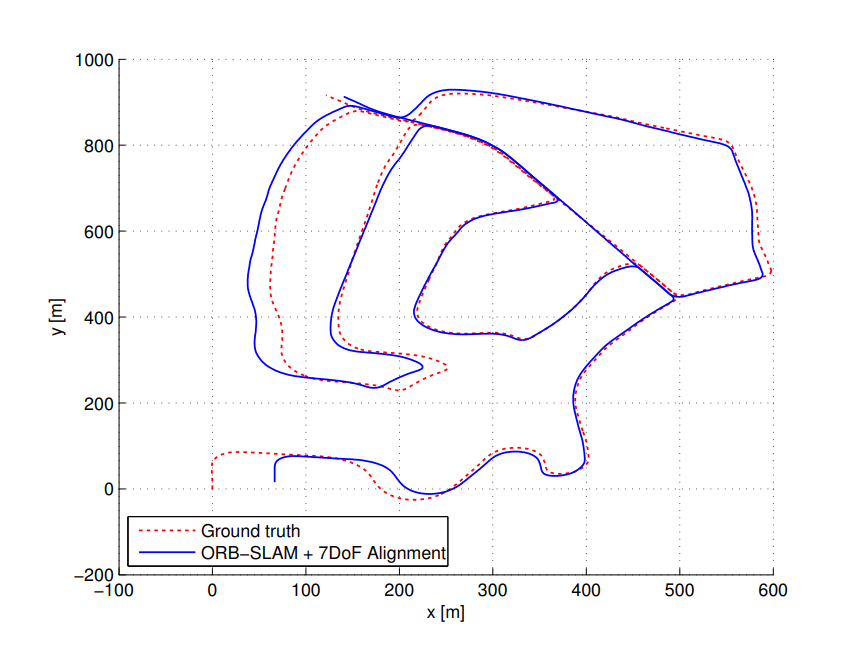
\includegraphics[width=0.4\textwidth]{Reports/3-Analysis-of-Baselines/images/orb02.png} % Replace with your image file
        \label{fig:orb-slam11}
    }
    \hspace{0.05\textwidth} % Space between subfigures
    \subfigure[Sequence 08]{
        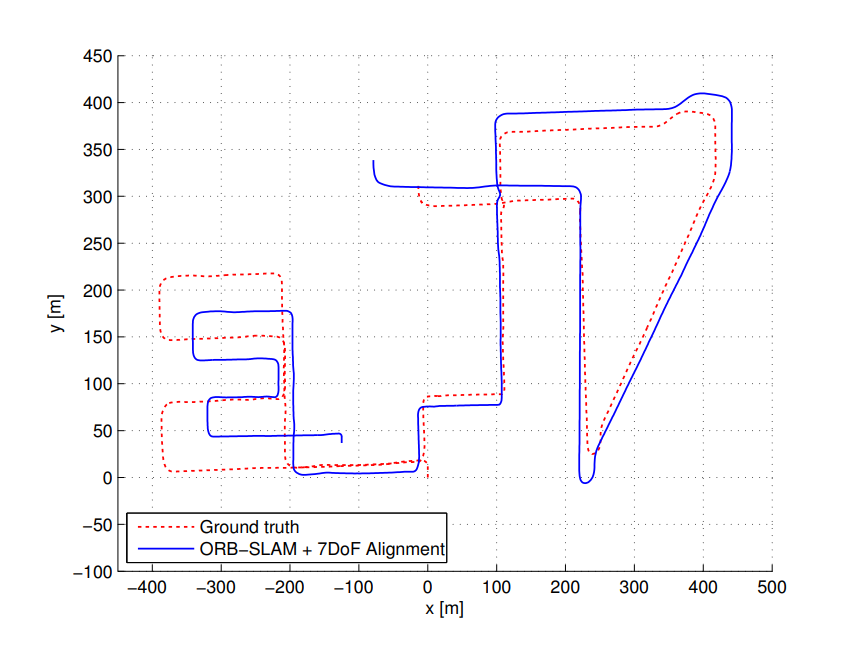
\includegraphics[width=0.4\textwidth]{Reports/3-Analysis-of-Baselines/images/orb08.png} % Replace with your image file
        \label{fig:orb-slam13}
    }
    \hspace{0.05\textwidth} % Space between subfigures
    \subfigure[Sequence 10]{
        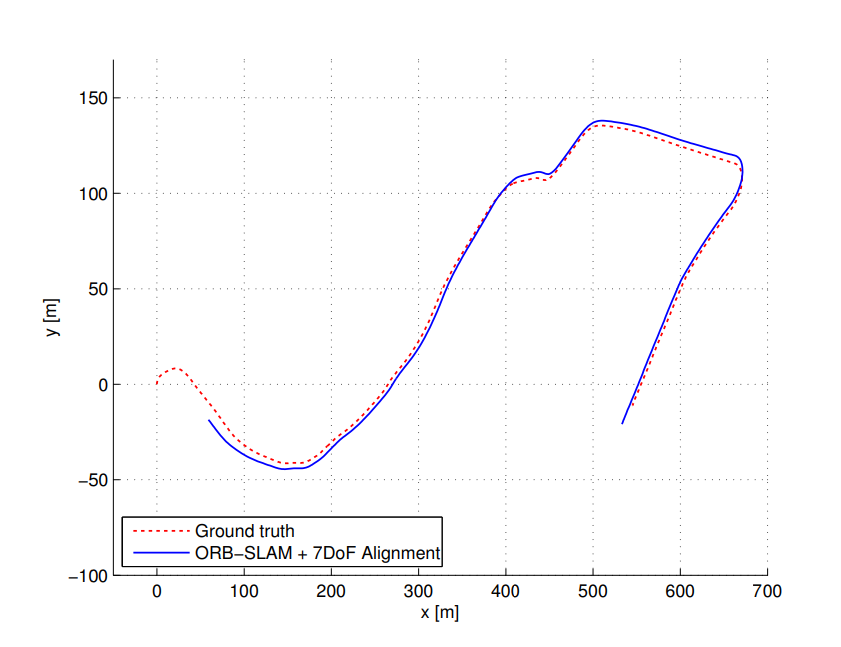
\includegraphics[width=0.4\textwidth]{Reports/3-Analysis-of-Baselines/images/orb10.png} % Replace with your image file
        \label{fig:orb-slam14}
    }
    \caption{Results of ORB-SLAM2 on KITTI Sequences 02, 08, 10. It is interesting to note the performances around loop crossings and long-tail trackings.}
    \label{fig:orb-slam2}
\end{figure}

\subsubsection{TartanVO}

TartanVO \cite{tartanvo} is the closest unimodal baseline to our work, as it uses the same two-frame formulation for odometry and is trained on the predecessor to the dataset we plan to use, TartanAir \cite{tartanair}. It also uses optical flow to establish correspondences between frames for pose estimation. Our goal is to match or exceed TartanVO’s performance when trained on only image data, and with the addition of LiDAR data, the performance should improve significantly as LiDAR provides crucial information, enabling 3D grounding and more accurate pose estimation.

The intrinsic metric we want to test against for TartanVO is their flow loss. Since we also plan on using flow as a method or correspondence computation, we analyze the effects of learning from a flow pre trained flow model, GMFlow, and how this affects the motion prediction.

\begin{figure}[htbp]
    \centering
    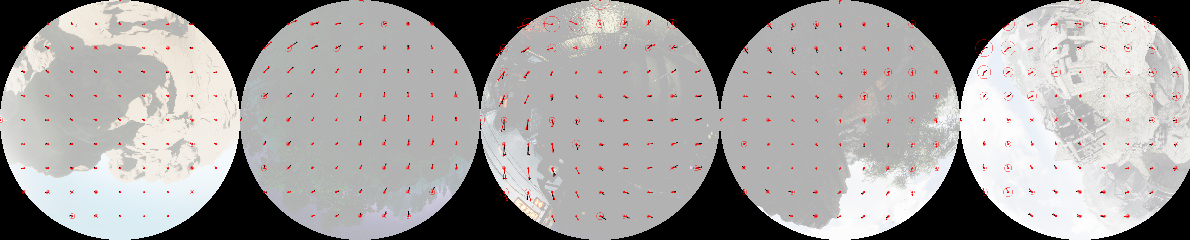
\includegraphics[width=8cm]{Reports/3-Analysis-of-Baselines/images/tartanvo/flow_img.png}
    \caption{Example intermediate flow visualizations from TartanVO}
    \label{fig:tvo-flow-img}
\end{figure}

\begin{figure}[htbp]
    \centering
    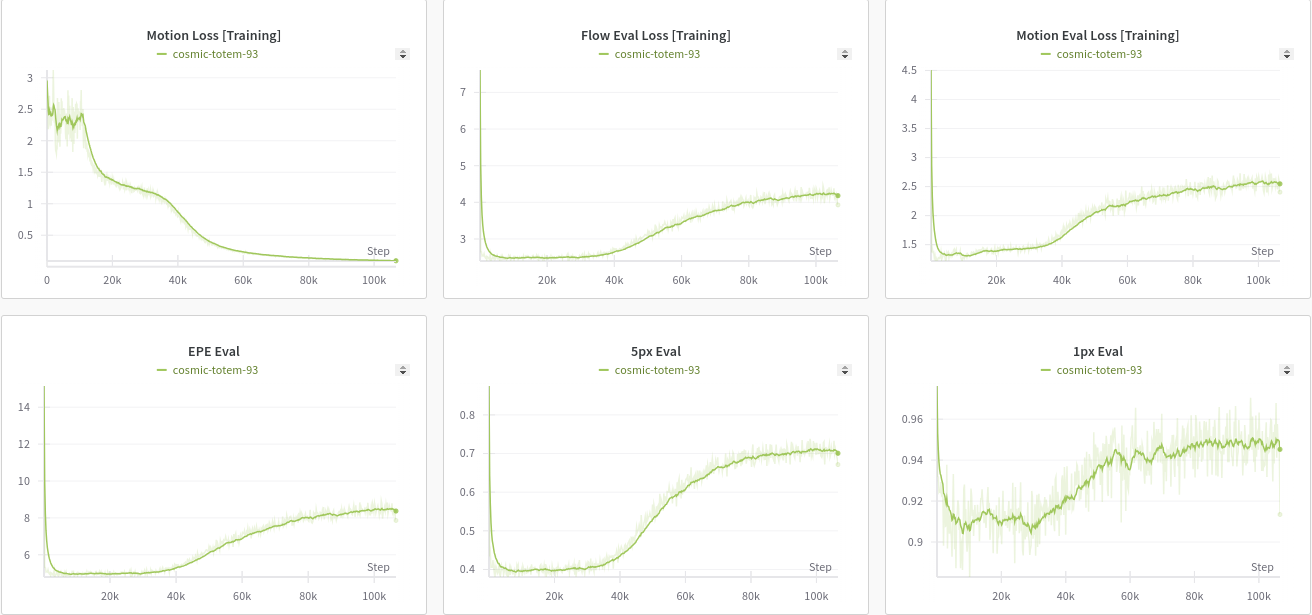
\includegraphics[width=8cm]{Reports/3-Analysis-of-Baselines/images/tartanvo/flow_loss.png}
    \caption{TartanVO motion and flow metrics during validation}
    \label{fig:tvo-flow-loss}
\end{figure}

\begin{figure}[htbp]
    \centering
    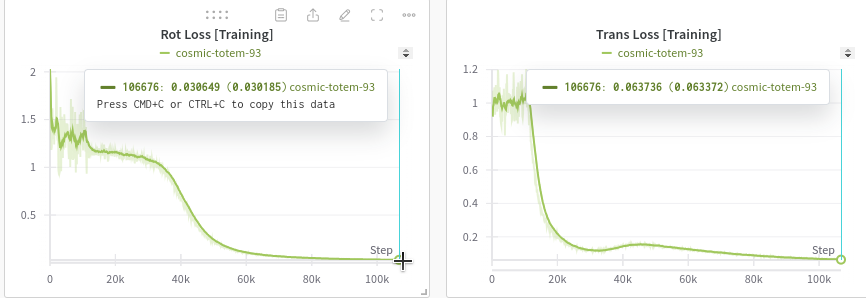
\includegraphics[width=8cm]{Reports/3-Analysis-of-Baselines/images/tartanvo/rot_trans_loss.png}
    \caption{TartanVO motion losses for rotation and translation}
    \label{fig:tvo-rot-trans}
\end{figure}

As shown in Figure \ref{fig:tvo-flow-loss}, we see that flow has an interesting relationship with the overall motion loss. The model is initialized with pre-trained flow and is trained using MSE on the motion. We see in the first plot that training motion loss starts off small and decreases, and in the second plot the flow validation loss starts off small, and in the third plot, the motion validation plot starts off small. This shows that flow can be a strong inductive bias to initialize odometry. More interestingly, as training progresses and the model overfits, we see that the training motion loss decreases while the validation motion and flow losses increase, showing that there is a tight correlation between the model's ability to perform optical flow and its ability to predict pose.

Another test we wanted to do with TartanVO is checking the scales of the rotation and translation components of the loss. The overall training objective in the sum of the rotation and translation losses and, as shown in Figure \ref{fig:tvo-rot-trans}, the rotation loss seems to be lower than the translation. We will need to balance these two losses properly to achieve better performance, or the model will be biased toward learning rotations over translations.

\subsection{LiDAR Odometry Methods}
We evaluated two LiDAR odometry methods: a classical approach, which is a variant of ICP SLAM that utilizes ScanContext for loop detection and miniSAM for loop closure, and a learning-based method, EfficientLO-Net \cite{eff-lo-net}. The evaluations of both methods are presented in the following sub-sections. 

\subsubsection{ICP-SLAM}
A SLAM pipeline, evaluated using only poses as states, was tested with ICP SLAM for odometry, Scan Context for loop detection, and miniSAM-based graph optimization on the KITTI dataset. The entire trajectory was empirically assessed to understand the pipeline's performance. For ICP, random downsampling with 7000 points was used, while the parameters for Scan Context were set to: Ring = 20, Sector = 60, and 30 ring key candidates. 

Figure \ref{fig:icp-kitti-2} illustrates the pipeline's performance on KITTI trajectory 2, with a loop closure threshold of 0.11. In this case, the loop was correctly detected, and the trajectory was optimized, aligning with the expected performance. Figures \ref{fig:icp-kitti-8} show the performance on KITTI trajectory 8 with loop detection thresholds of 0.07 and 0.20, respectively. In this case, either no loop was detected or a false loop was identified. This suggests that Scan Context may struggle with loop detection in scenarios where there is a significant change in lane level, as observed in KITTI trajectory 8.

\begin{figure}[htbp]
    \centering
    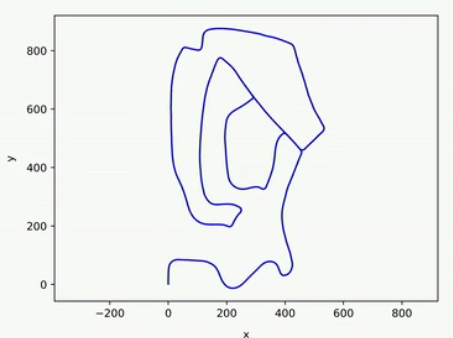
\includegraphics[width=4cm]{Reports/3-Analysis-of-Baselines/images/ICP-SLAM/KITTI_loop2.png}
    \caption{ICP SLAM on Trajectory 2: Loop Detected}
    \label{fig:icp-kitti-2}
\end{figure}

\begin{figure}[htbp]
    \centering
    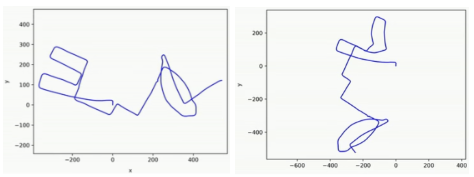
\includegraphics[width=8cm]{Reports/3-Analysis-of-Baselines/images/ICP-SLAM/kitti-08.png}
    \caption{ICP SLAM on Trajectory 8: Left - Threshold 0.007, Right - Threshold 0.20}
    \label{fig:icp-kitti-8}
\end{figure}

\subsubsection{EfficientLO-Net}
Efficient LO-Net was evaluated as a learning-based lidar odometry method. The average translational error(\%) for sequences 00-05, over distances ranging from 100 to 800 meters, remained below 0.55\%, with the rotational error (deg/m) not exceeding 0.38. In contrast, for Sequence 08, the translational error increased to 1.14\%. Sequence 08 presents a particularly challenging urban environment, characterized by sharp turns, intersections, dynamic obstacles like moving vehicles, and varying road structures. These elements likely posed significant challenges for Efficient LO-Net, making it difficult to maintain accurate feature associations across frames. The presence of dynamic objects and the complex structure of the scene likely contributed to increased translational drift, as the model may have struggled to differentiate between the vehicle’s motion and that of surrounding objects and to manage occlusions and variable feature distributions in the lidar data.



\begin{figure}[t]
\centering
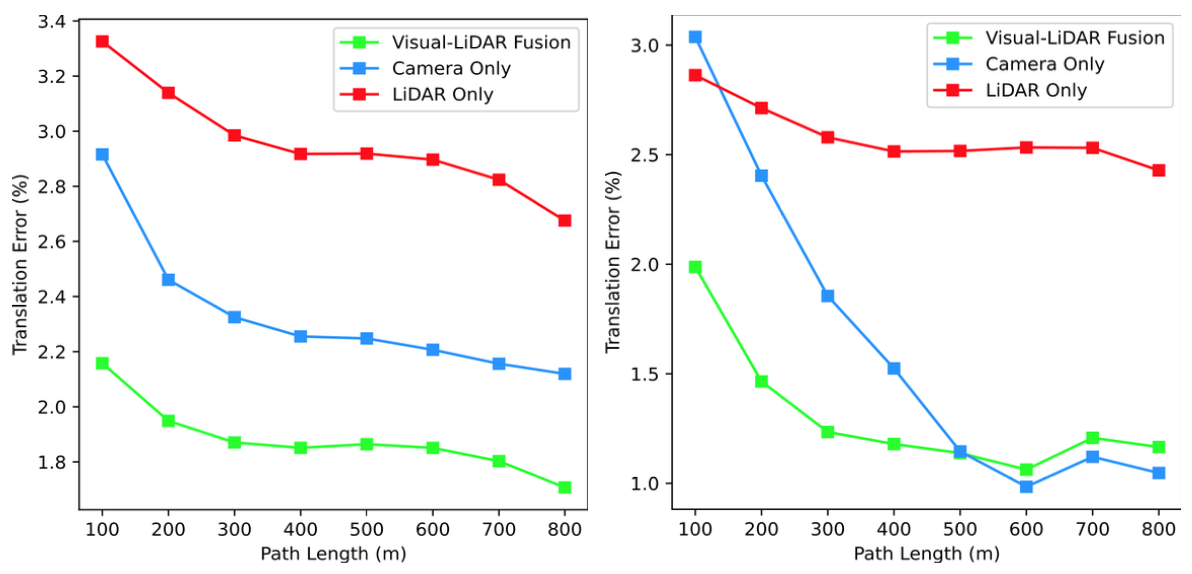
\includegraphics[width=\columnwidth]{Reports/3-Analysis-of-Baselines/images/HVLO-ablations.png}
\caption{
    Translation errors averaged across sub-sequences of various lengths (100, 200, ..., 800 meters) within sequences 09 and 10 of the KITTI dataset. The performance results for the LiDAR-only method (red lines), camera-only method (blue lines), and LiDAR-camera fusion method (green lines) are displayed.
}
\vspace{-0.4cm}
\label{fig:multimodal-plot}
\end{figure}
\begin{figure}[t]
\centering
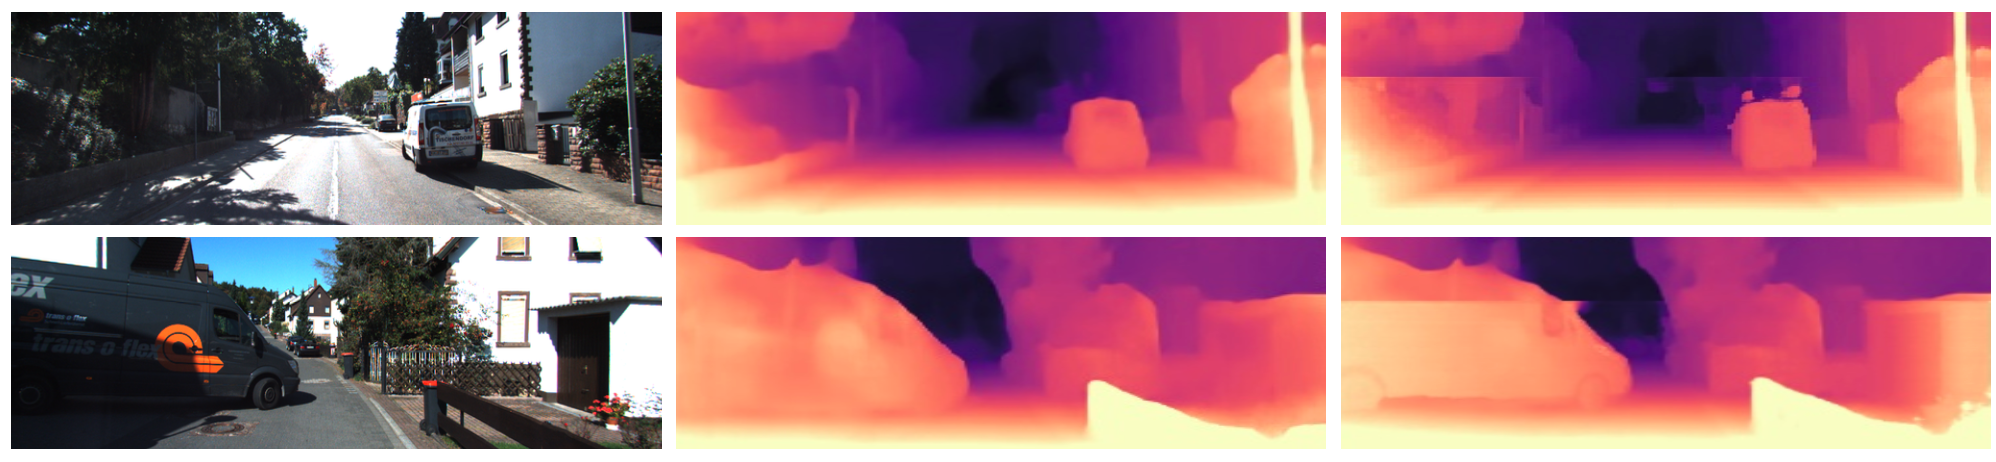
\includegraphics[width=\columnwidth]{Reports/3-Analysis-of-Baselines/images/HVLO-ablations-pic.png}
\caption{
    Effectiveness of visual-LiDAR fusion for better estimation of dense depth map. Each row contains one example of the improvement in RGB image frame, DepthNet estimation, fusion result, respectively. Top row: attachments to the roof of the vehicle exist in the fused map where DepthNet is not able to estimate it. Bottom row: Vehicle boundaries are more noticeable and DepthNet is fooled due to graphics at the side hood of the van.
}
\vspace{-0.4cm}
\label{fig:multimodal-pic}
\end{figure}

\subsection{Multimodal Odometry Methods}

\subsubsection{H-VLO}
Since H-VLO~\cite{hvlo} demonstrates robust performance by effectively combining LiDAR and camera modalities, we leverage its structure to examine the benefits of integrating these modalities in a LiDAR-camera fusion method. This approach is contrasted with single-modality methods that rely solely on either LiDAR or camera data, allowing us to isolate and understand the unique advantages provided by each data source as well as their combined effect. Figure~\ref{fig:multimodal-plot} illustrates the translational errors averaged across sub-sequences of various lengths (100, 200, ..., 800 meters) within sequences 09 and 10 of the KITTI dataset. The performance results for the LiDAR-only method (red lines), camera-only method (blue lines), and LiDAR-camera fusion method (green lines) are displayed.

The LiDAR-only method, represented by the red lines, yields the least accurate trajectory estimates, showing that depth information alone is insufficient for precise motion estimation and mapping, particularly in scenarios where detailed semantic cues are essential for distinguishing objects and understanding scene context. Without these semantic details, the LiDAR-only approach struggles, resulting in higher translational errors, particularly over longer sub-sequence lengths.

On the other hand, the camera-only method (blue lines) performs notably better, benefiting from the rich semantic information inherent in RGB images. Camera data captures texture, color, and object detail, which enhances scene interpretation and aids in predicting object movements and scene transitions. As a result, the camera-only method achieves significantly lower translational errors compared to the LiDAR-only approach, especially in sub-sequences where scene complexity demands higher contextual understanding. However, despite its advantages, the camera-only method still encounters limitations in environments where depth perception is crucial but cannot be accurately derived from monocular RGB images alone.

By combining the semantic information from camera data with the depth and structural detail from LiDAR data, the LiDAR-camera fusion approach (green lines) harnesses the strengths of both modalities. This fusion achieves superior results by providing a more comprehensive representation of the environment: LiDAR contributes precise spatial geometry, while the camera supplies detailed scene semantics. Leveraging the fusion structure within H-VLO, the LiDAR-camera fusion method demonstrates the lowest translational errors across all sub-sequence lengths, suggesting that integrating these complementary data sources not only improves trajectory accuracy but also enhances robustness in complex environments with varying levels of occlusion, lighting, and scene intricacies.

\subsubsection{DVLO}
Most learning-based approaches, such as H-VLO~\cite{hvlo}, focus on feature-level fusion but often fail to capture the fine-grained pixel-to-point correspondences required for precise pose estimation. These approaches are further challenged by the inherent structural differences between sparse LiDAR points and dense camera pixels, resulting in data misalignment that limits the effectiveness of multi-modal fusion.

To address these limitations, DVLO~\cite{dvlo} introduces a novel local-to-global fusion network with bi-directional structure alignment, specifically designed to enhance the integration of LiDAR and visual features for more accurate pose estimation. In particular, DVLO clusters neighboring visual information in 2D images by projecting LiDAR depth data onto the 2D image plane. This clustering enables effective alignment of LiDAR points with visually similar pixels, improving spatial consistency.

As shown in Figure~\ref{fig:dvlo}, pixels with similar texture information (yellow regions) are clustered by calculating the point-wise cosine similarity with designated cluster centers (red dots). This approach ensures that visual information is more cohesively grouped with corresponding depth data, leading to a more refined fusion of LiDAR and visual features and ultimately resulting in enhanced pose estimation accuracy.

\begin{figure}[htbp]
    \centering
    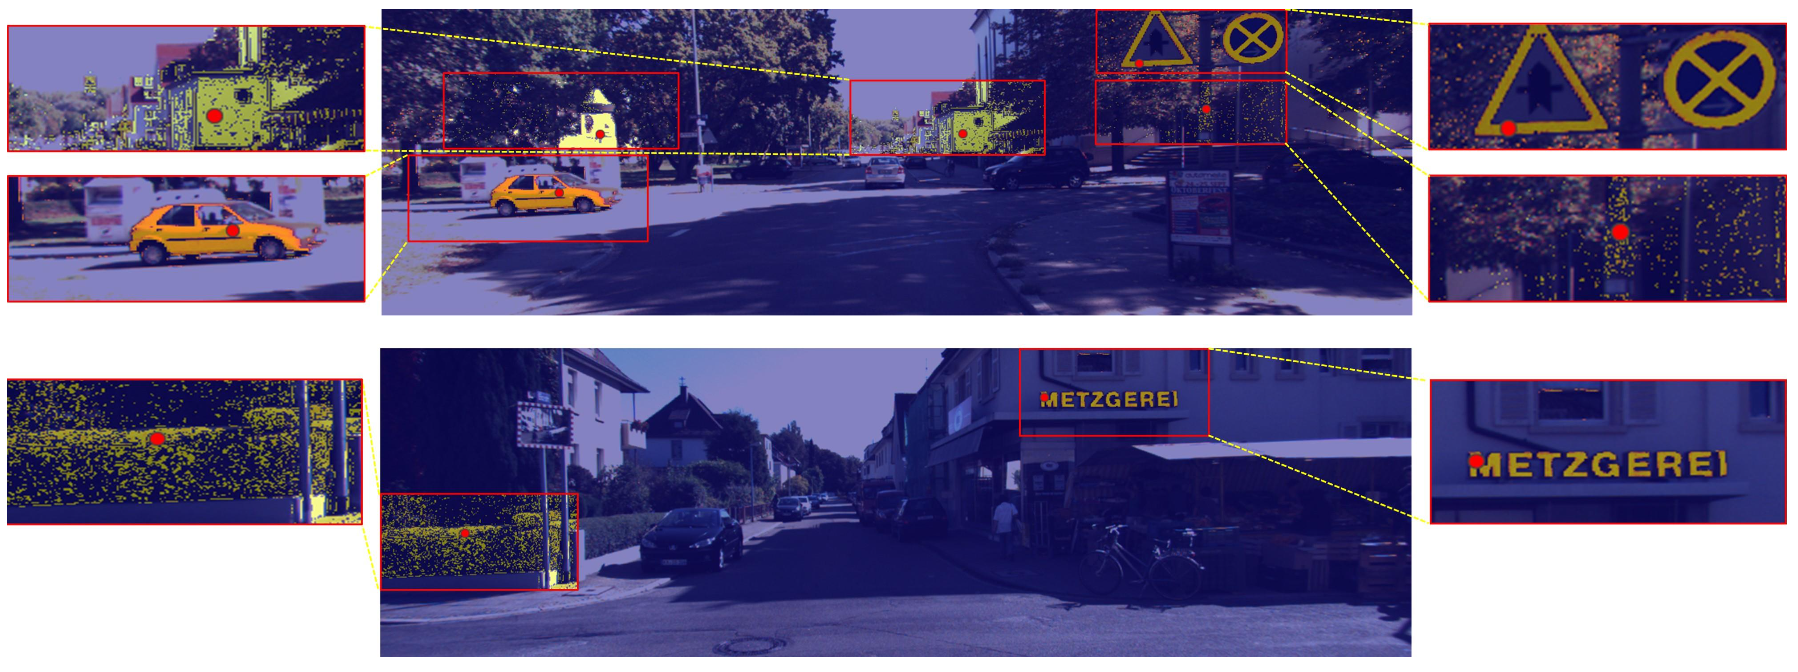
\includegraphics[width=8cm]{Reports/3-Analysis-of-Baselines/images/dvlo.png}
    \caption{Visualization of DVLO's local clustering-based fusion mechanism within a certain cluster. Red points indicate the 2D positions of cluster centers. The yellow regions are clustered pixels around each center.}
    \label{fig:dvlo}
\end{figure}

\subsubsection{SDV-LOAM}
SDV-LOAM (Semi-Direct Visual-LiDAR Odometry and Mapping) \cite{sdv-loam} was evaluated as one of the classical multimodal baselines. It is a robust odometry method that effectively combines visual and LiDAR data for accurate pose estimation and mapping. The system addresses common challenges in visual-LiDAR fusion by incorporating a semi-direct visual odometry approach and an adaptive sweep-to-map LiDAR odometry.

The visual module of SDV-LOAM employs a novel technique that directly extracts high-gradient pixels where 3D LiDAR points project for tracking, avoiding the need for explicit 3D-2D depth association. To handle large-scale differences between matching frames, it uses a point matching with propagation method, which propagates points from a host frame to an intermediate keyframe closer to the current frame. This approach significantly reduces scale differences and improves tracking accuracy.

On the LiDAR side, SDV-LOAM introduces an adaptive sweep-to-map optimization method that dynamically chooses between optimizing 3 horizontal degrees of freedom (DOF) or 6 full DOF pose based on the richness of geometric constraints in the vertical direction. This adaptive approach helps reduce pose estimation drifts, particularly in the vertical direction. Some interesting results of the interesting inference runs are shown in figure \ref{fig:sdv-loam}.

\begin{figure}[h!]
    \centering
    \subfigure[Sequence 13]{
        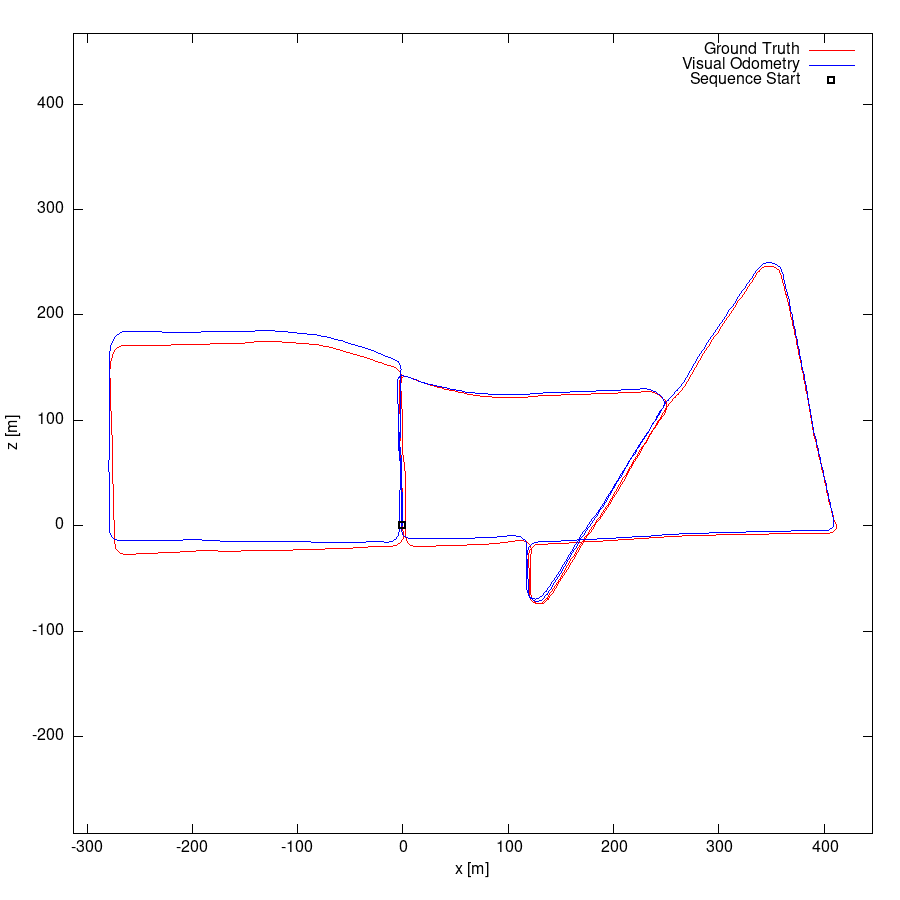
\includegraphics[width=0.4\textwidth]{Reports/3-Analysis-of-Baselines/images/sdv13.png} % Replace with your image file
        \label{fig:sdv13}
    }
    \hspace{0.05\textwidth} % Space between subfigures
    \subfigure[Sequence 14]{
        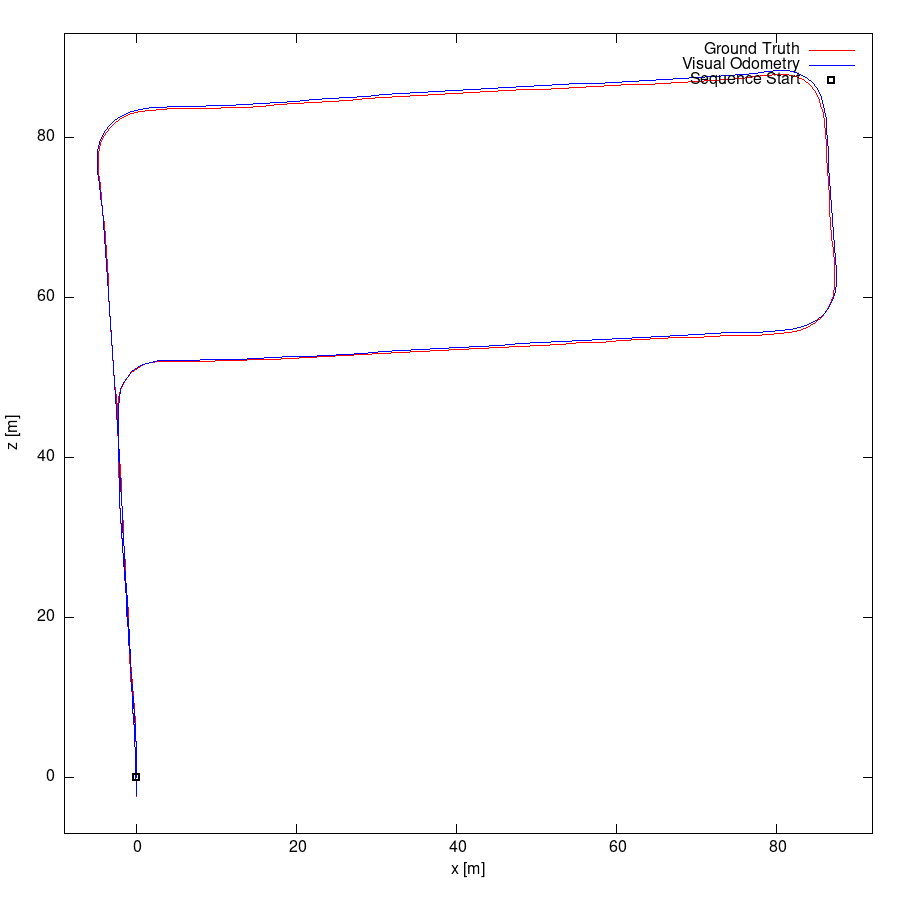
\includegraphics[width=0.4\textwidth]{Reports/3-Analysis-of-Baselines/images/sdv14.png} % Replace with your image file
        \label{fig:sdv14}
    }
    \hspace{0.05\textwidth} % Space between subfigures
    \subfigure[Sequence 15]{
        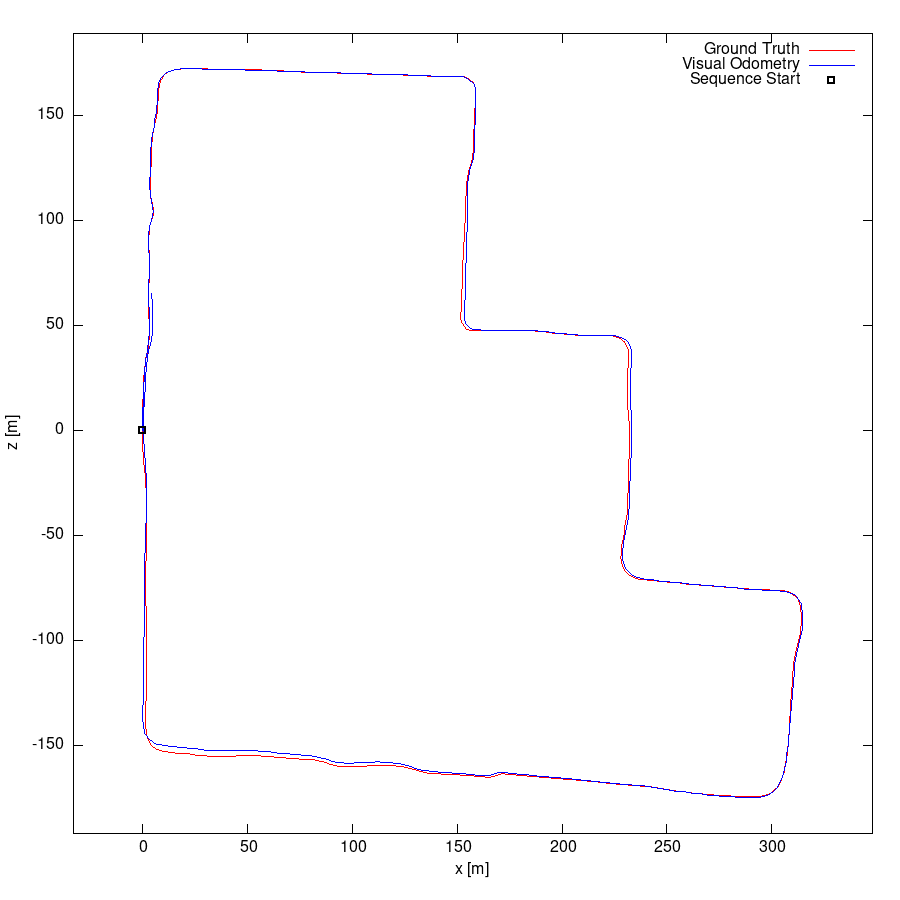
\includegraphics[width=0.4\textwidth]{Reports/3-Analysis-of-Baselines/images/sdv15.png} % Replace with your image file
        \label{fig:sdv15}
    }
    \caption{Results of SDV-LOAM on KITTI Sequences 13, 14, 15 \cite{KITTI}.}
    \label{fig:sdv-loam}
\end{figure}

\clearpage
\section{Proposed Model}
\begin{figure*} [t]
    \centering
    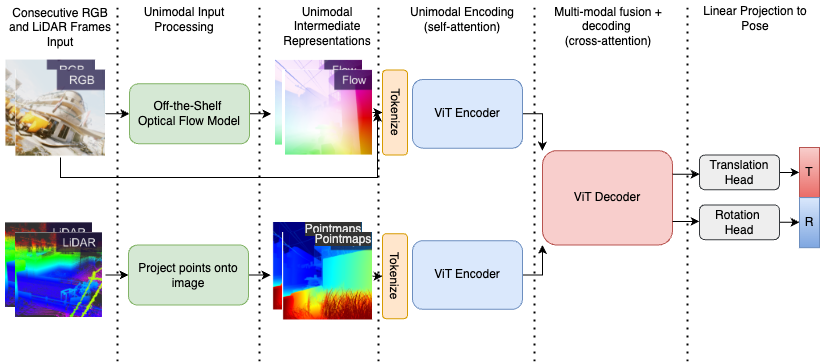
\includegraphics[width=0.95\linewidth]{Reports/2-Baselines-and-Model-Proposal/images/VOL_model.png}
    \caption {The VOL model diagram. Given RGB and LiDAR frames from two consecutive timesteps, the model computes optical flow and aligns the LiDAR points to the point map. These intermediate representations are then processed by the separate encoder and combined into a decoder, and lastly sent through translation and rotation heads to recover pose.}
    \label{fig:model-diagram}
\end{figure*}

\subsection{Overall model structure}
The model first consists of a preprocessing step for both the RGB images and LiDAR point clouds. The images are sent through an optical flow regression model to get an intermediary flow representation, and the point clouds are projected onto the image to enforce explicit alignment between the 2D pixels and the corresponding 3D points. These processed modalities are then sent through their respective ViT encoders and then combined with a ViT decoder and a projection head to output pose. The model diagram is presented in Figure \ref{fig:model-diagram}. Some key changes from out initial proposed model include projecting our LiDAR points into pointmaps instead of depth, and adding the initial RGB images to the flow as input.

% \clearpage

\subsection{Unimodel Processing}
\subsubsection{RGB}
The key information we seek from the RGB input is the presence of strong visual features that allow us to match between frames and establish correspondences. To achieve this, we process the images by running them through a flow model, which computes optical flow to provide dense correspondences between frames. TartanVO trains its odometry model solely using a flow model as its encoder, so we have evidence that this approach retrains information needed for odometry. We then concatenate the two frames with their corresponding flow to form the final processed input from the RGB data to retain all information for the decoder. We use GMFlow \cite{gmflow} as our pretrained flow model.

\subsubsection{LiDAR}
We preprocess the LiDAR point cloud by projecting it onto the image space, such that the 3D points are in the shape of the image but contain $(x,y,z)$ values instead of $(R, G, B)$ as shown in DVLO \cite{dvlo}. This "point-map" 3D representation has been shown to be very effective in relating 2D RGB images to 3D points, as seen in works like DUSt3R \cite{dust3r}. Since the pointmap is in the same shape as the RGB image, the points can be concatenated, establishing strong correspondence between RGB pixels and their corresponding LiDAR points. We can then use the same encoder as used for the RGB images on these point maps, thus making the shared space between the two modalities more homogeneous.

\subsection{Multimodal Decoder}
The decoder is a ViT decoder architecture that performs cross-attention between the intermediate flow and pointmap encodings. This mechanism will allow for effective global information sharing between the two modalities. The output of this module is then sent to separate heads for rotation and translation similar to the TartanVO architecture \cite{tartanvo}, enabling precise recovery of pose parameters. We have also tried using a ResNet backbone as the decoder model, and we observed that the model performance is similar. We believe the strong pixel-wise correspondences of the concatenated flow, RBG, and LiDAR data enables for easier modality fusion, making the exact architecture of the decoder less significant.

\subsection{Loss Functions}
% Describe both your primary task loss and three possible auxiliary losses that might improve performance.  Justify your choices.

The primary objective used to train the model will be a simple mean-squared error on the predicted translation and rotation.

\begin{equation} \label{eq:sim1}
L_{pose} = \|\hat{T} - T\| + \|\hat{R} - R\|
\end{equation}

This is based on the objective used for TartanVO \cite{tartanvo}, but uses absolute translation error instead of up-to-scale error since we wish to determine absolute pose. 

An auxiliary loss that we believe greatly helps in inducing relevant biases for the model are optical flow. 

\begin{equation}
    L_{flow} = \sum_{i=1}^{N}||\mathbf{f}_{gt} - \mathbf{f}_i||_1
\end{equation}


Without the flow loss, we show that the pretrained RGB flow model will forget its flow capabilities, losing its inductive biases for finding correspondences. This auxiliary loss ensures that the model retains that flow knowledge while also learning to estimate pose. This is shown in Figure \ref{fig:flow_supervision}


\begin{figure}[h!]
    \centering
    \begin{tabular}{ccc} % Two columns
        % First row
        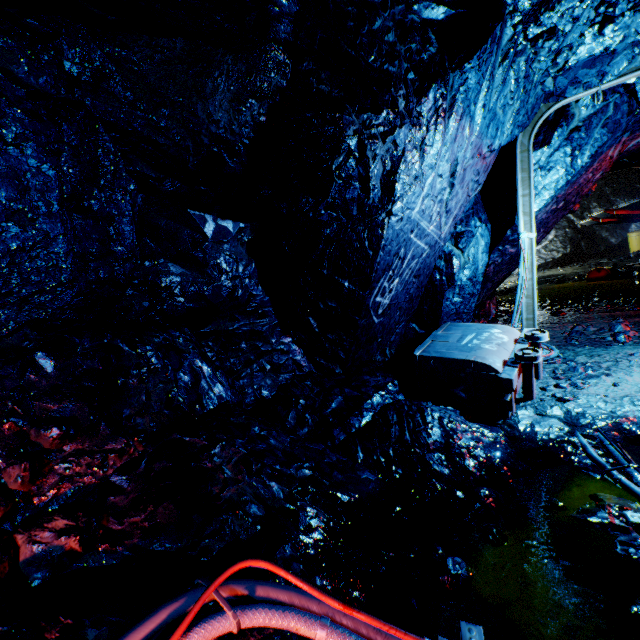
\includegraphics[width=0.12\textwidth]{Reports/4-Final-Report/images/flow_supervision/step_1_1.png} & 
        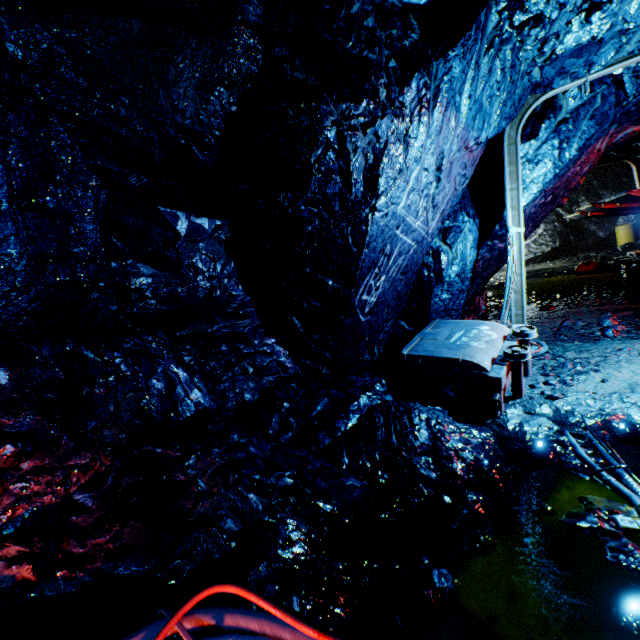
\includegraphics[width=0.12\textwidth]{Reports/4-Final-Report/images/flow_supervision/step_1_2.png} & 
        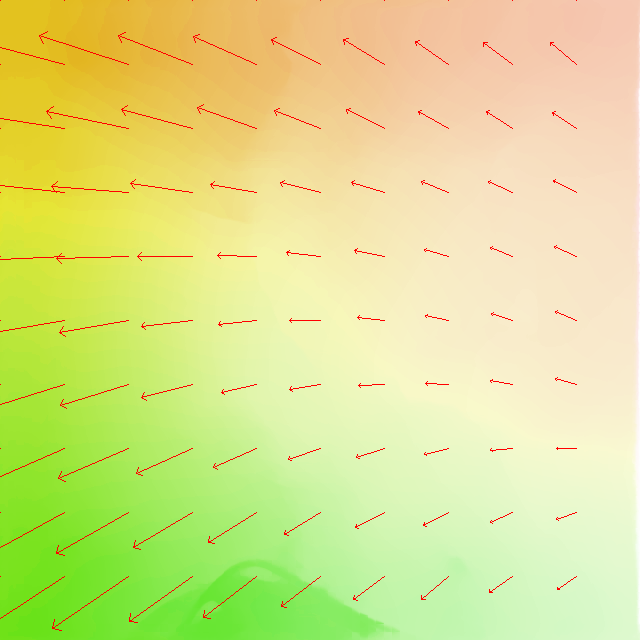
\includegraphics[width=0.12\textwidth]{Reports/4-Final-Report/images/flow_supervision/good_flow.png}\\ 
        
        % Second row
        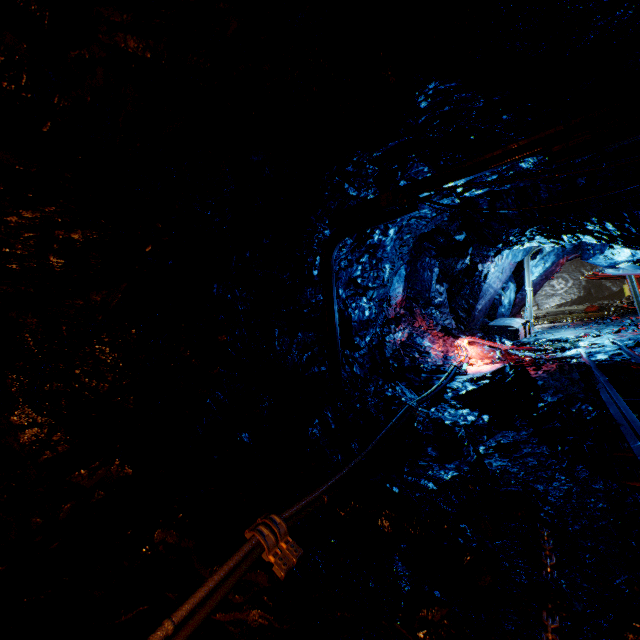
\includegraphics[width=0.12\textwidth]{Reports/4-Final-Report/images/flow_supervision/step5000_1.png} & 
        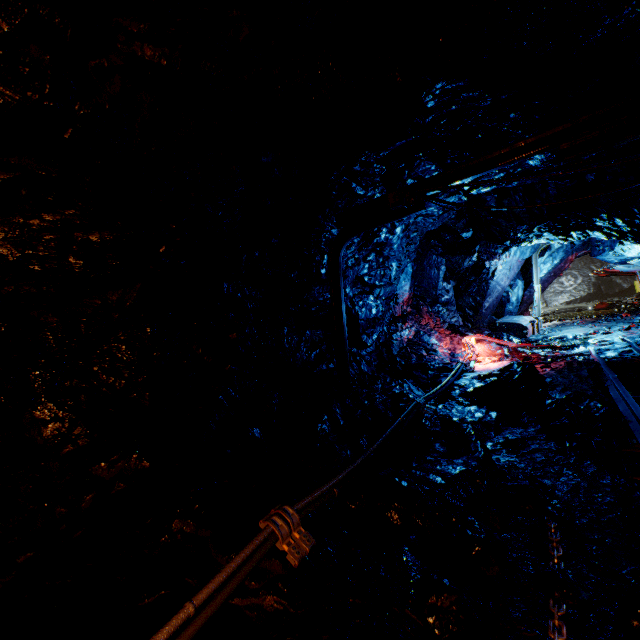
\includegraphics[width=0.12\textwidth]{Reports/4-Final-Report/images/flow_supervision/step_5000_2.png} & 
        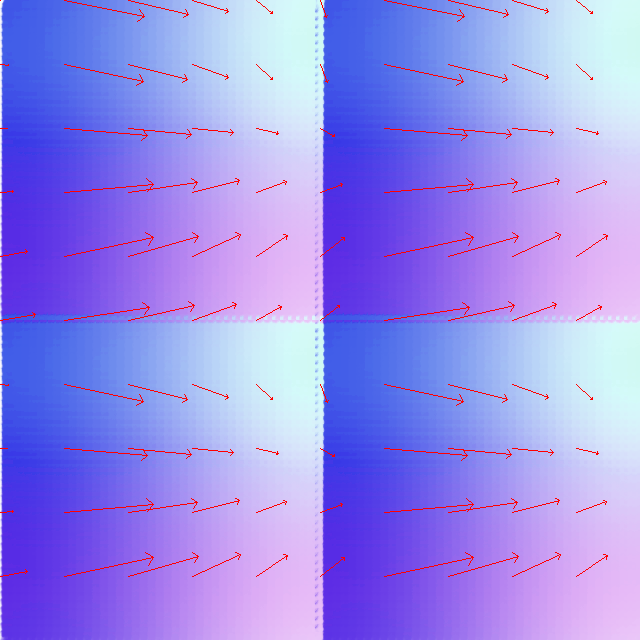
\includegraphics[width=0.12\textwidth]{Reports/4-Final-Report/images/flow_supervision/bad_flow.png}\\ 
    \end{tabular}
    \caption{The top row shows the model intermediate flow output during training at step 1 when training start. We observe that the pretrained flow model outputs reasonable flow. The bottom row shows the flow output after 5000 steps without flow supervision. We see that the flow output degrades, and we also observed that the model's performance on odometry also drops.}
    \label{fig:flow_supervision}
\end{figure}


In combination, the final loss will look as follows:

\begin{equation}
    L_{total} = L_{pose} + \lambda_1*L_{flow}
\end{equation}

We hypothesize that the composition of these relevant auxiliary tasks will induce a robust and accurate objective for odometry.

\subsection{Changes to training data}

Given that we trained solely on a synthetic dataset, some key augmentations to the training data were required to enable better generalization. For the LiDAR point clouds, dropout was applied to simulate their inherent sparsity, as real-world LiDAR data often lacks points for every pixel due to occlusions and sensor limitations. Additionally, random padding was introduced to the RGB images during training, enabling the model to handle variable aspect ratios and better generalize to diverse real-world RGB data. These augmentations were crucial for bridging the gap between synthetic and real-world scenarios. Visualizations of the final training data can be seen in Figure \ref{fig:augmentations}

\begin{figure}[h!]
    \centering
    \begin{tabular}{cc} % Two columns
        % First row
        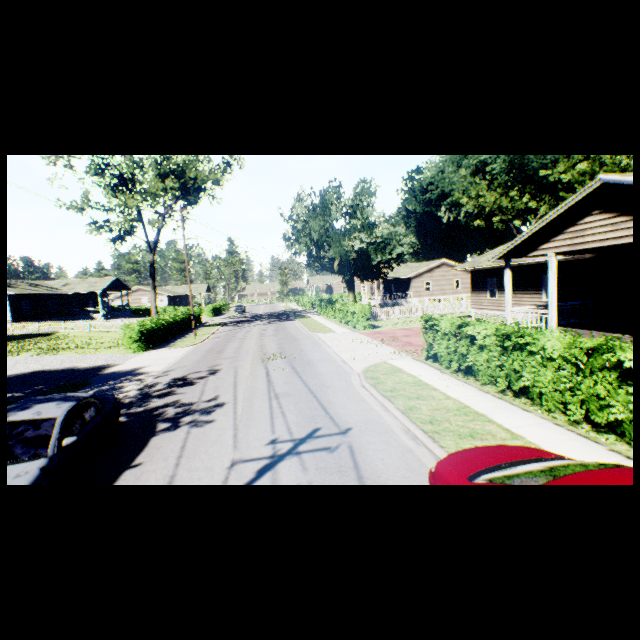
\includegraphics[width=0.2\textwidth]{Reports/4-Final-Report/images/augmentations/pad_1.png} & 
        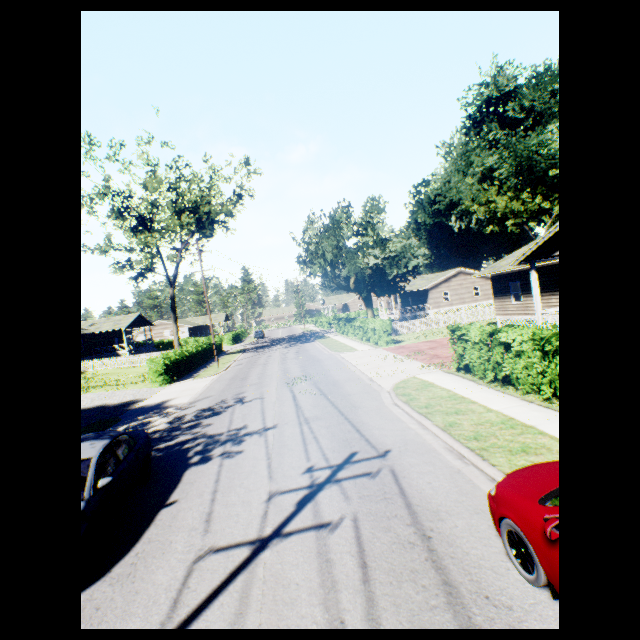
\includegraphics[width=0.2\textwidth]{Reports/4-Final-Report/images/augmentations/pad_2.png} \\ 
        
        % Second row
        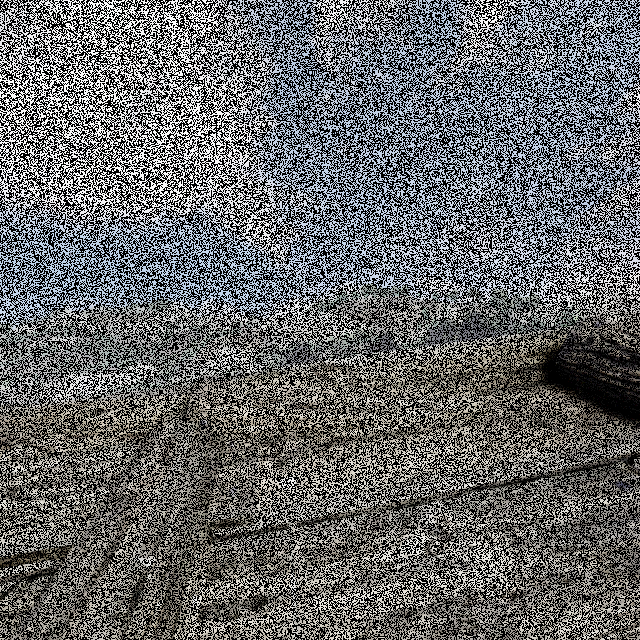
\includegraphics[width=0.2\textwidth]{Reports/4-Final-Report/images/augmentations/dropout_1.png} & 
        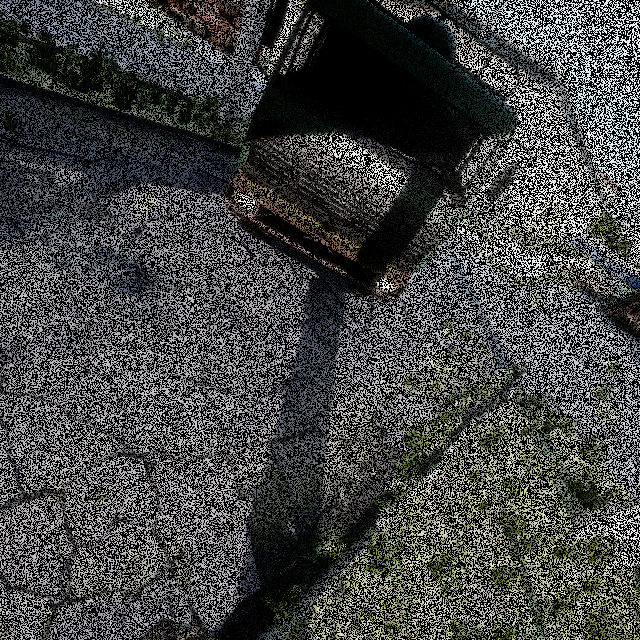
\includegraphics[width=0.2\textwidth]{Reports/4-Final-Report/images/augmentations/dropout_2.png} 
    \end{tabular}
    \caption{The top row shows the random padding augmentation to enable random aspect ratio inputs. The bottom row shows LiDAR dropout applied to RGB images for visualization.}
    \label{fig:augmentations}
\end{figure}

\subsection{Hyperparameters and their effects}

Key hyperparameters were the loss alphas, the addition of the flow loss, and the training curriculum.

\clearpage

    % \begin{tabular}{lllll|cc|cc|cc|cc}
    % \linewidth
    % \toprule
    % \multicolumn{5}{l|}{\multirow{2}[0]{*}{\textbf{Method}}} & \multicolumn{2}{c|}{06} & \multicolumn{2}{c|}{07} & \multicolumn{2}{c|}{09} & \multicolumn{2}{c}{10} \\
    %      &      &      &      &      & $t_{rel}$ & $r_{rel}$ & $t_{rel}$ & $r_{rel}$ & $t_{rel}$ & $r_{rel}$ & $t_{rel}$ & $r_{rel}$\\
    % \midrule
    % \multicolumn{13}{l}{\it{Visual Odometry Methods:}} \\
    % \midrule
    % \multicolumn{5}{l|}{ORB-SLAM (-)} & 18.68 & 0.26 & 10.96 & 0.37 & 15.3 & \textbf{0.26} & 3.71 & \textbf{0.3}  \\
    % \multicolumn{5}{l|}{TartanVO (*)} & 4.72 & 2.95 & 4.32 & 3.41 & 6.0 & 3.11 & 6.89 & 2.73 \\
    % \midrule
    % \multicolumn{13}{l}{\it{LiDAR Odometry Methods:}} \\
    % \midrule
    % \multicolumn{5}{l|}{ICP-SLAM (-)} & 1.95 & 1.59 & 5.17 & 3.35 & 6.93 & 2.89 & 8.91 & 4.74  \\
    % \multicolumn{5}{l|}{LO-Net (*)} & 1.04 & 0.69 & 0.71 & 0.50 & 2.12 & 0.77 & 1.80 & 0.93 \\
    % \midrule
    % \multicolumn{13}{l}{\it{Multimodal Odometry Methods:}} \\
    % \midrule
    % \multicolumn{5}{l|}{H-VLO (*)} & 0.75 & 0.30 & 0.79 & 0.48 & 1.89 & 0.34 & 1.36 & 0.43 \\
    % \multicolumn{5}{l|}{DVLO (*)} & \textbf{0.33} & \textbf{0.17} & \textbf{0.46} & \textbf{0.33} & 0.85 & 0.36 & 0.88 & 0.46 \\
    % \multicolumn{5}{l|}{DV-LOAM (-)} & 0.65 & 0.33 & 0.51 & \textbf{0.33} & 0.73 & 0.32 & 0.87 & 0.38 \\
    % \multicolumn{5}{l|}{SDV-LOAM (-)} & 0.50 & 0.27 & 0.84 & 0.53 & \textbf{0.63} & 0.34 & \textbf{0.68} & 0.41 \\
    % {\it{Proposed Method:}} \\
    % \midrule
    % \multicolumn{5}{l|}{VOL} & 0.75 & 0.30 & 0.79 & 0.48 & 1.89 & 0.34 & 1.36 & 0.43 \\
    % % \multicolumn{5}{l|}{DVLO (*)} & \textbf{0.33} & \textbf{0.17} & \textbf{0.46} & \textbf{0.33} & 0.85 & 0.36 & 0.88 & 0.46 \\
    % % \multicolumn{5}{l|}{DV-LOAM (-)} & 0.65 & 0.33 & 0.51 & \textbf{0.33} & 0.73 & 0.32 & 0.87 & 0.38 \\
    % % \multicolumn{5}{l|}{SDV-LOAM (-)} & 0.50 & 0.27 & 0.84 & 0.53 & \textbf{0.63} & 0.34 & \textbf{0.68} & 0.41 \\
    % % \midrule
    % \bottomrule
    % \label{tab:results}
    % \end{tabular}


\clearpage
\section{Results (1 page)}
We evaluated the model architecture using the KITTI odometry dataset, primarily to benchmark its performance against other baselines.


\subsection{Required Steps}

\begin{itemize}
    \item \textbf{DataLoader:} To facilitate this evaluation, we developed a KITTI sequence loader to load the requested data sequences along with the specified sequence length. To ensure compatibility with the PyTorch DataLoader, we designed a pipeline that loads images, lidar point clouds, and calibration data. This data includes the extrinsics between the lidar and camera, which were used to transform the lidar information into the camera frame. Additionally, the camera intrinsics were provided as output, enabling the evaluation script to project lidar points onto the camera image.
    
    \item \textbf{Evaluation Script:} For model inference on the KITTI dataset, the input data needed to be correctly formatted. Since our training dataset images differed in shape from those in the KITTI dataset, we resized the images while maintaining the aspect ratio to match the model's required input shape. Figure 3 illustrates a KITTI image, while Figure 2 shows the reshaped input image fed into the model. Similarly, for the lidar input, we projected the lidar points onto the image plane using camera intrinsics. Afterward, the projected lidar points were rescaled to match the input shape of the model. Once this preprocessing was complete, we proceeded with model inference testing.
\end{itemize}   

\begin{figure}[t]
    \centering
    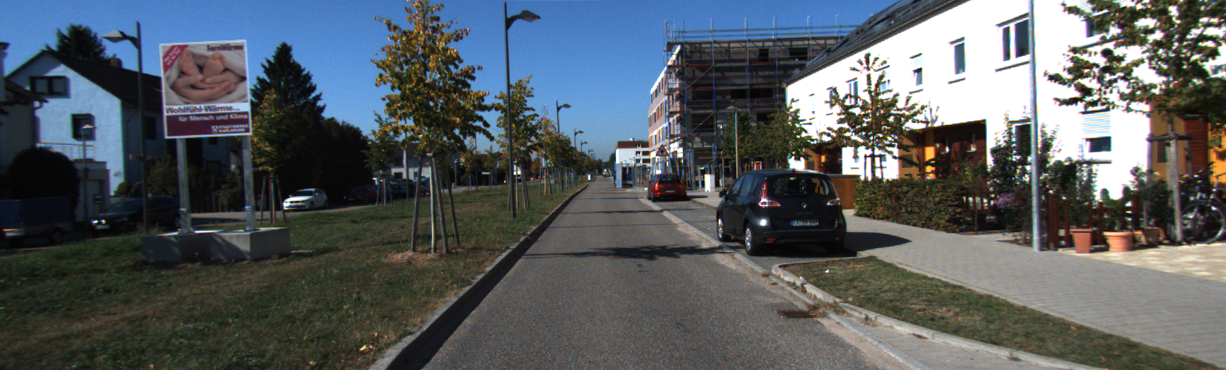
\includegraphics[width=1.0\linewidth]{Reports/4-Final-Report/images/results/kitti-0.png}
    \caption{KITTI Sequence 0, Image 1}
    \label{fig:kitti-img1}
\end{figure}

\begin{figure}[t]
    \centering
    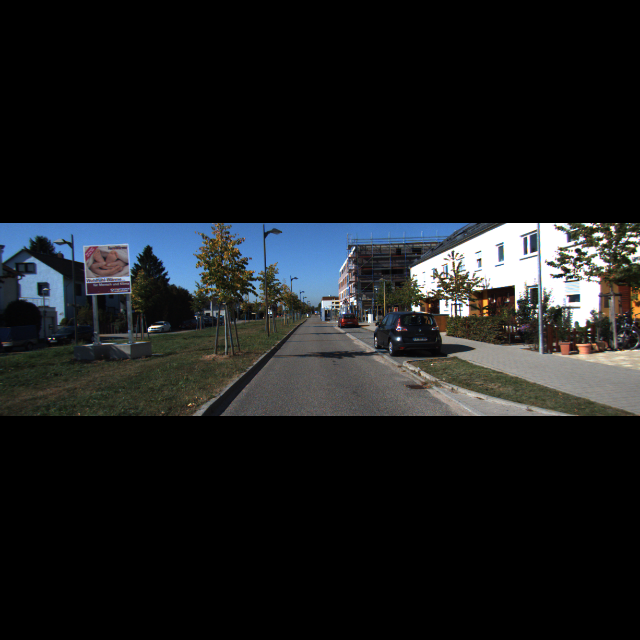
\includegraphics[width=1.0\linewidth]{Reports/4-Final-Report/images/results/vol_input-0.png}
    \caption{Processed Image for the model, Image 1}
    \label{fig:kitti-img1}
\end{figure}


\clearpage
\section{Analysis (2 pages)}
This section should include plots.  For example, how key metrics vary with a specific hyperparameter, task complexity, etc.

\subsection{Intrinsic Metrics}
The key intrinsic metric we measured was flow, which plays a crucial role in ensuring accurate correspondences between frames. It was essential to retain flow information during training while carefully balancing the extent to which the model focuses on odometry without forgetting flow. We achieved this balance through a carefully designed curriculum training strategy. Initially, we trained the model with the flow module frozen and no augmentations applied, allowing the model to focus on foundational learning. Subsequently, we introduced augmentations and unfroze the flow module, adding flow supervision to guide learning. This approach significantly improved model performance, as the flow outputs demonstrated that the model successfully learned the augmentations, developing some invariance to varying aspect ratios as shown in Figure \ref{}. Consequently, flow served as a valuable auxiliary measure for evaluating robustness to these augmentations. We observe that the flow loss also closely follows the odometry loss curve, indicating a strong correlation as shown in Figure \ref{fig:Flow_losses}.


\begin{figure}[h!]
    \centering
    \begin{tabular}{cc} % Two columns
        % First row
        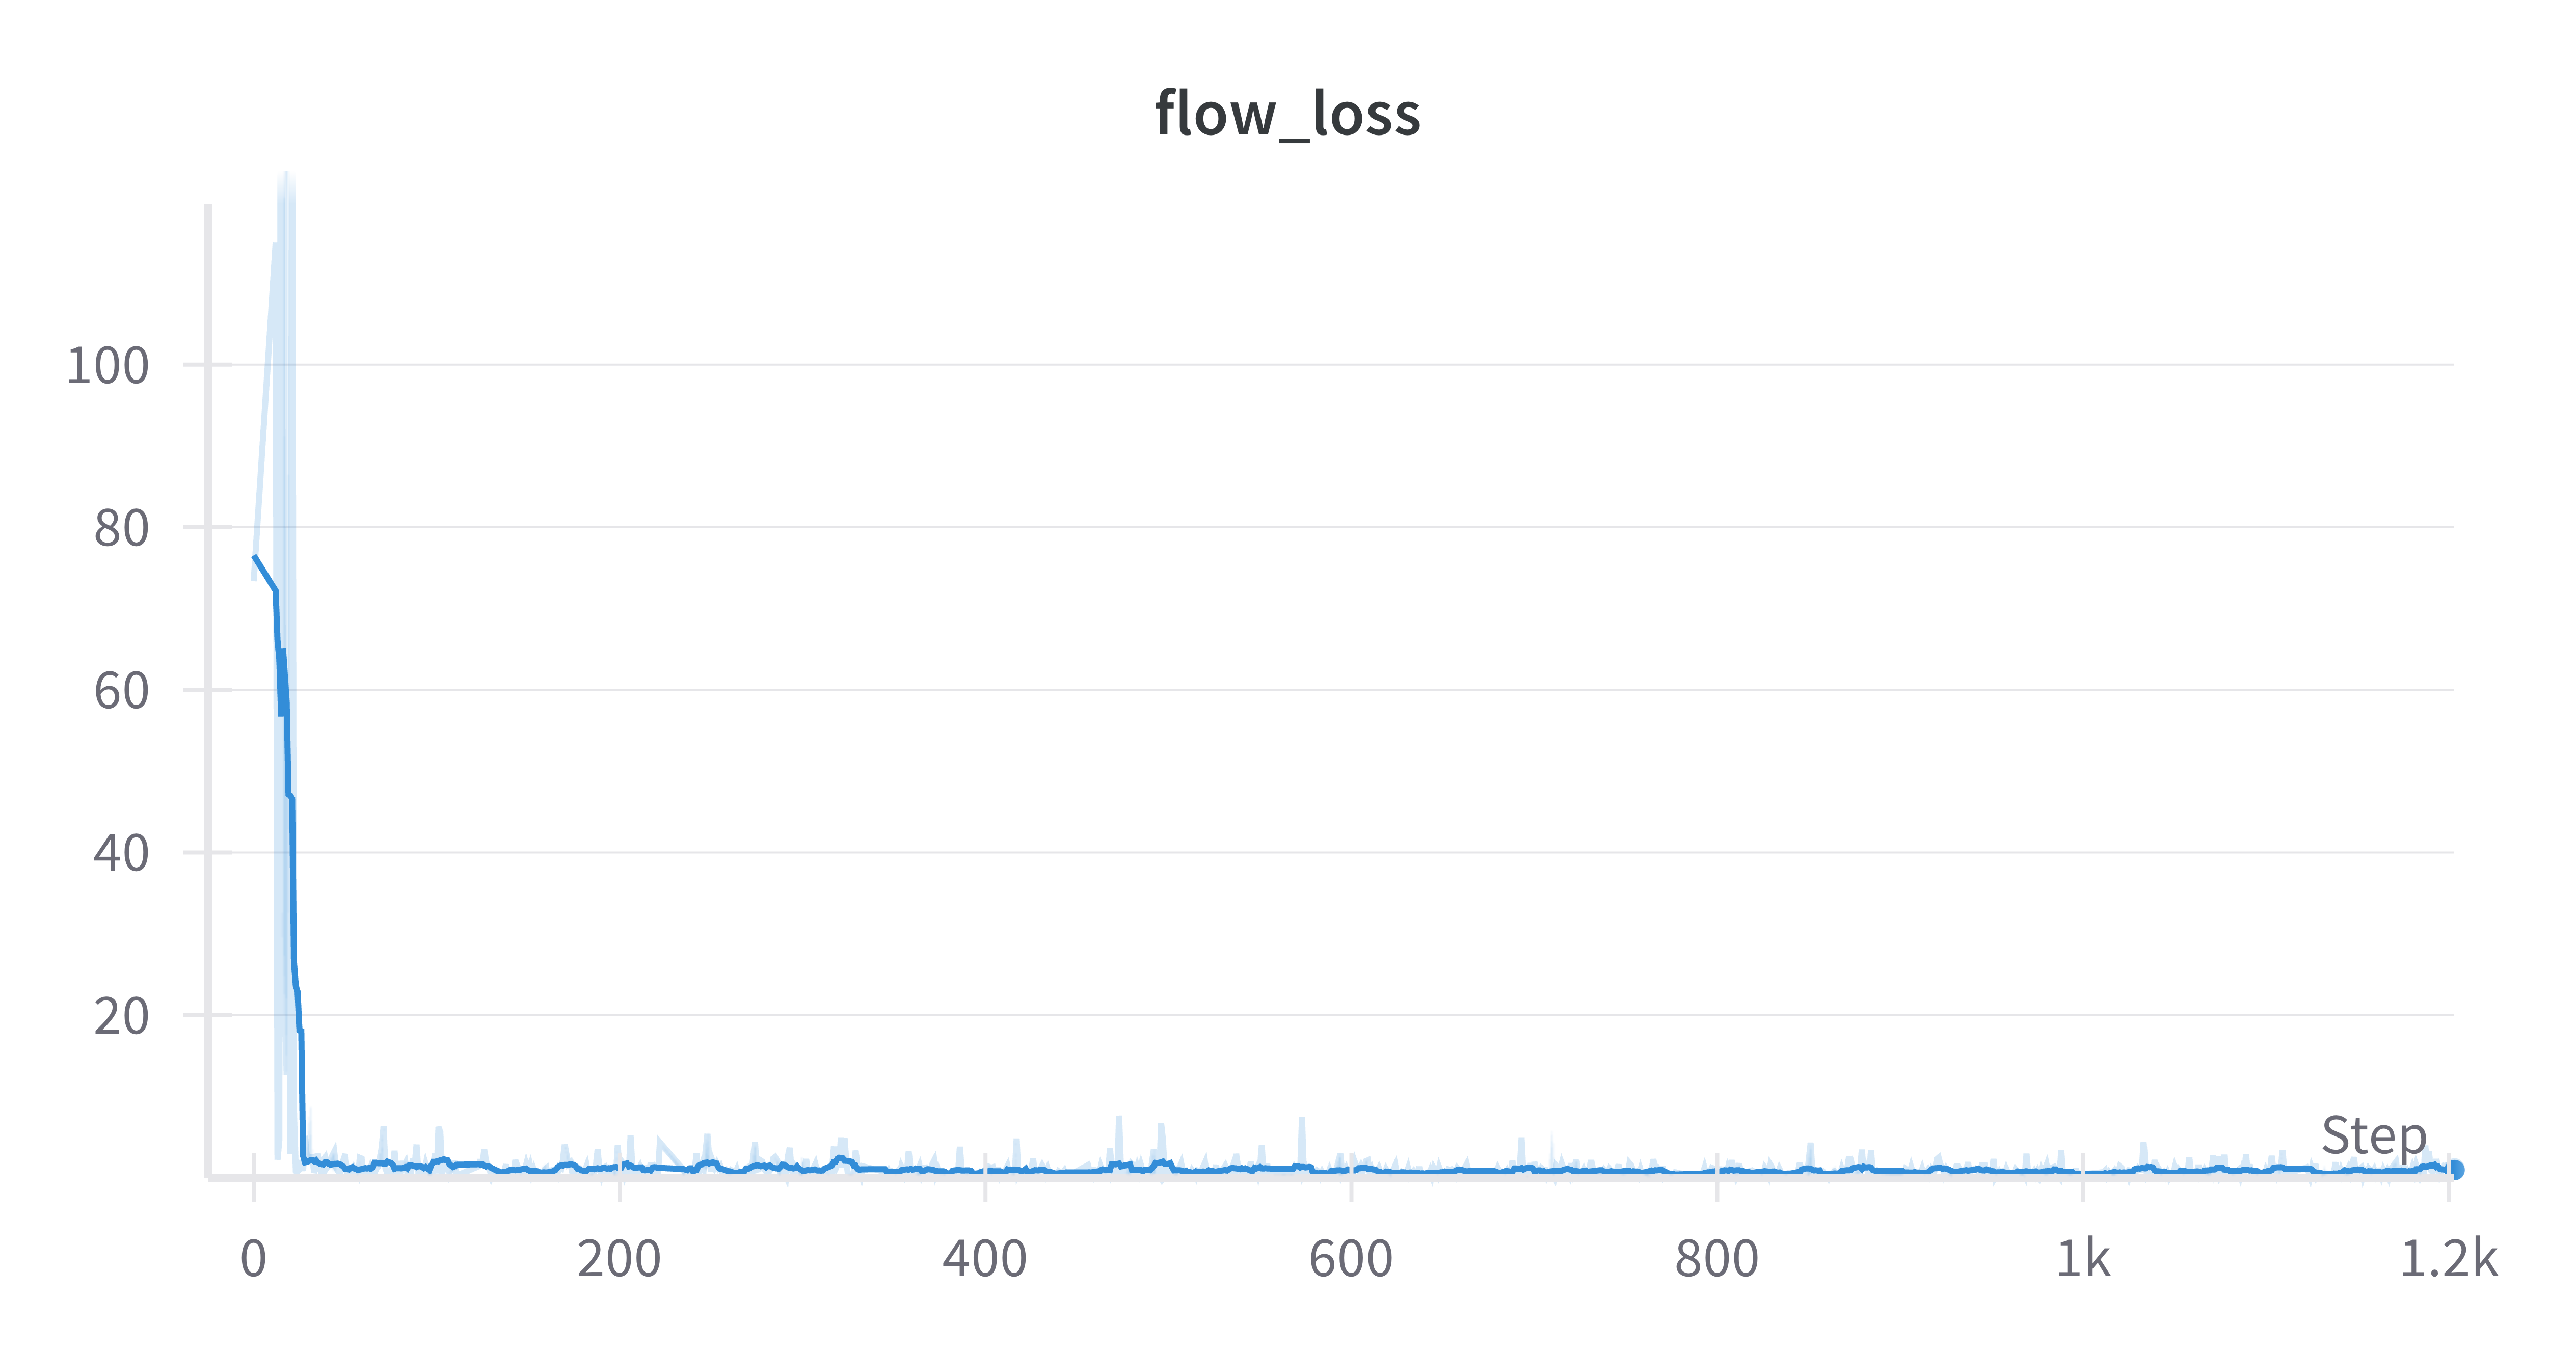
\includegraphics[width=0.22\textwidth]{Reports/4-Final-Report/images/intrinsic_metric/flow_loss.png} & 
        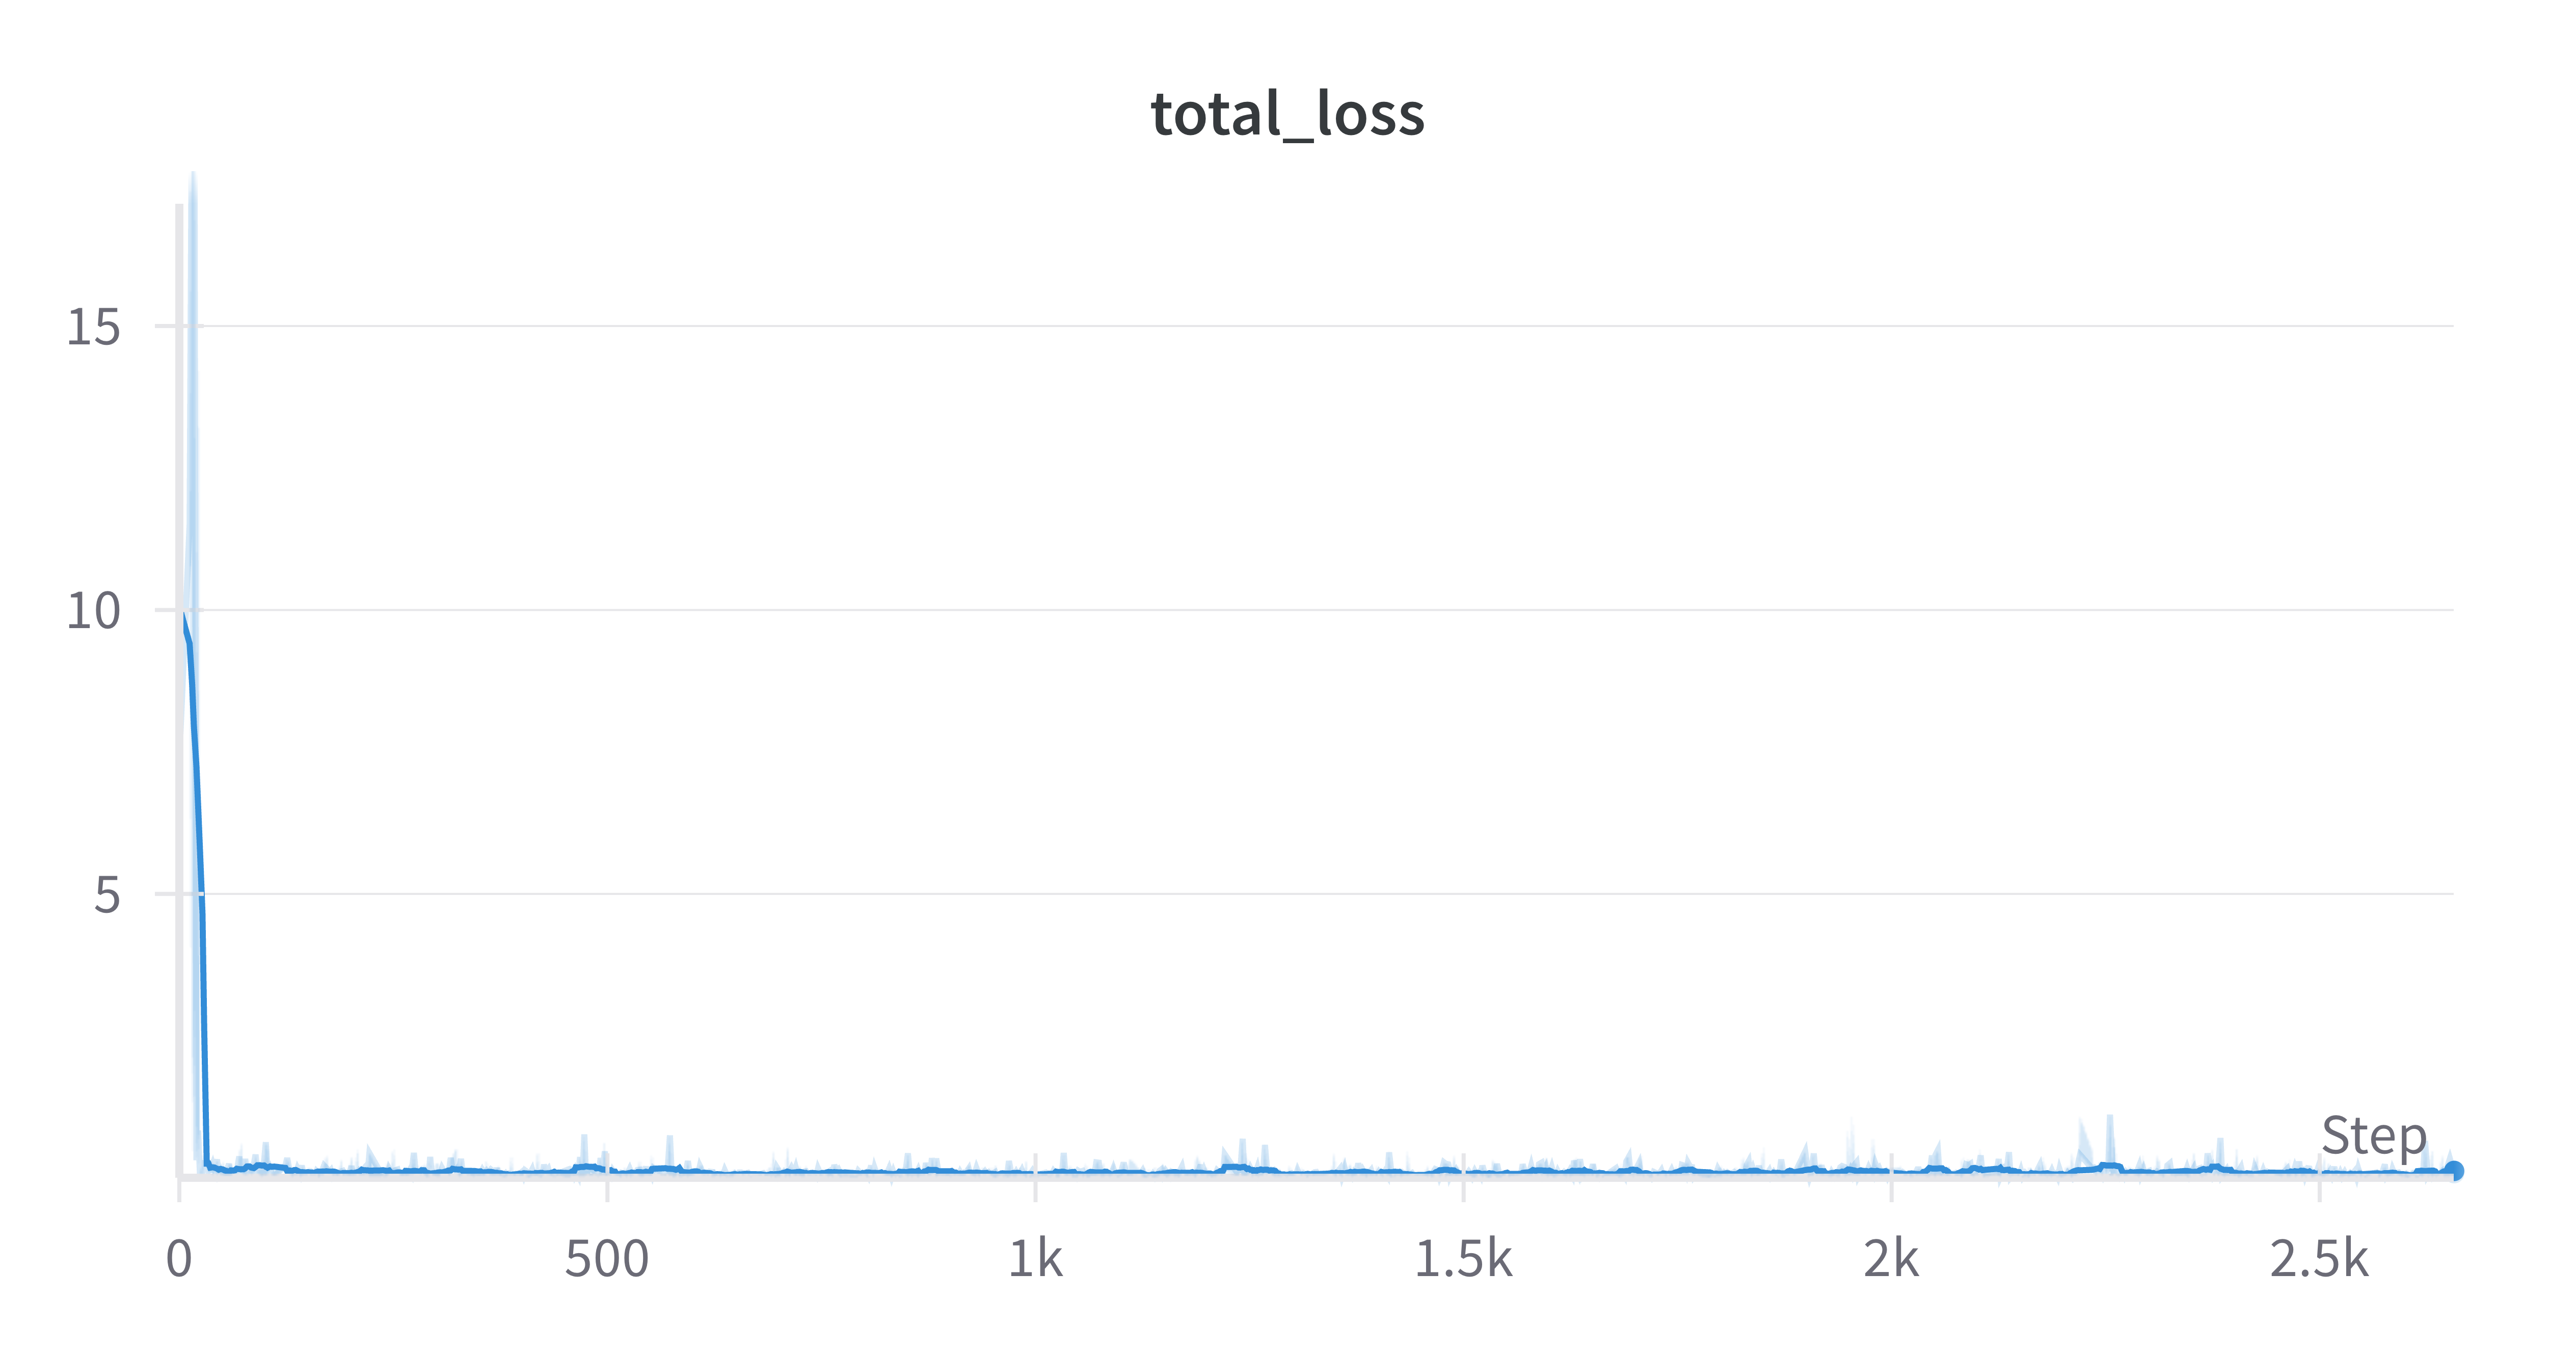
\includegraphics[width=0.22\textwidth]{Reports/4-Final-Report/images/intrinsic_metric/total_loss.png} \\ 
     
    \end{tabular}
    \caption{The first image shows the flow loss and the second image shows the total loss. Observe that both loss curves are highly correlated.}
    \label{fig:Flow_losses}
\end{figure}


\begin{figure}[h!]
    \centering
    \begin{tabular}{ccc} % Two columns
        % First row
        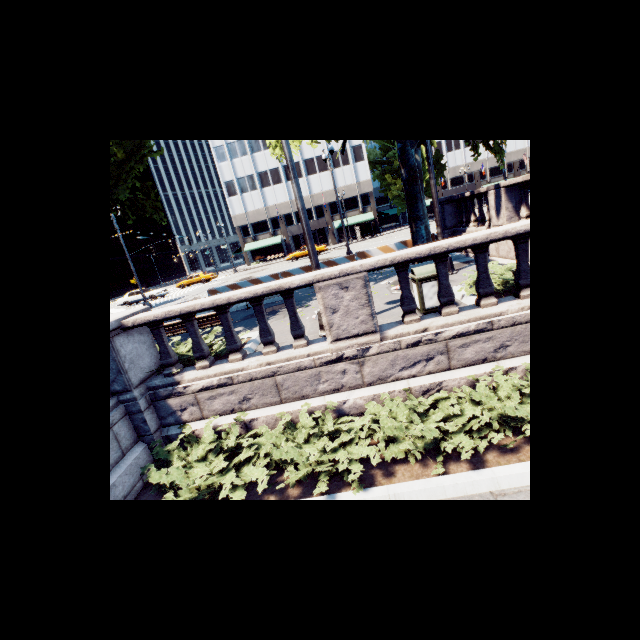
\includegraphics[width=0.22\textwidth]{Reports/4-Final-Report/images/intrinsic_metric/img_bad.png} & 
        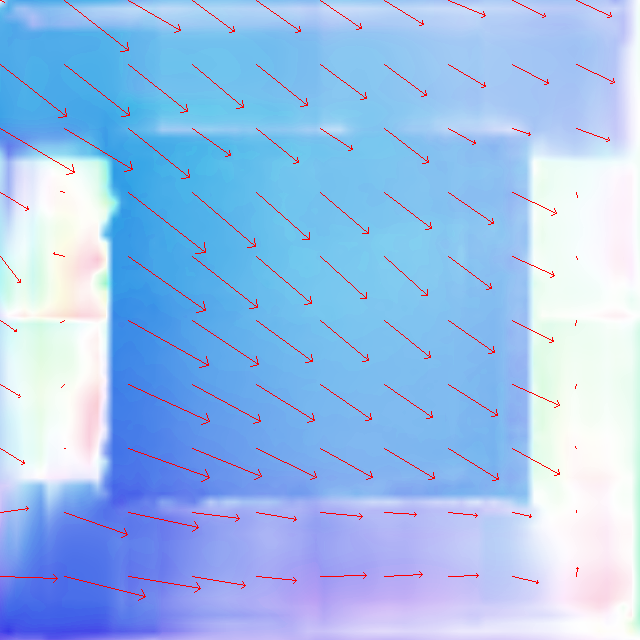
\includegraphics[width=0.22\textwidth]{Reports/4-Final-Report/images/intrinsic_metric/flow_bad.png}\\ 
        
        % Second row
        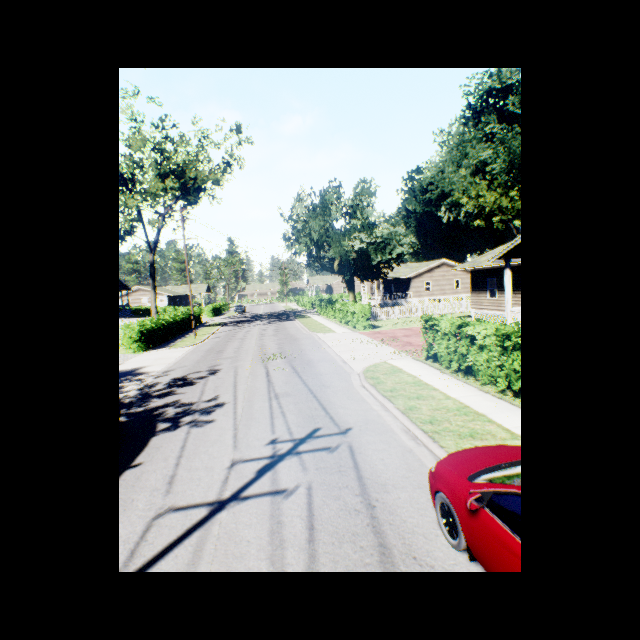
\includegraphics[width=0.12\textwidth]{Reports/4-Final-Report/images/intrinsic_metric/img1.png} & 
        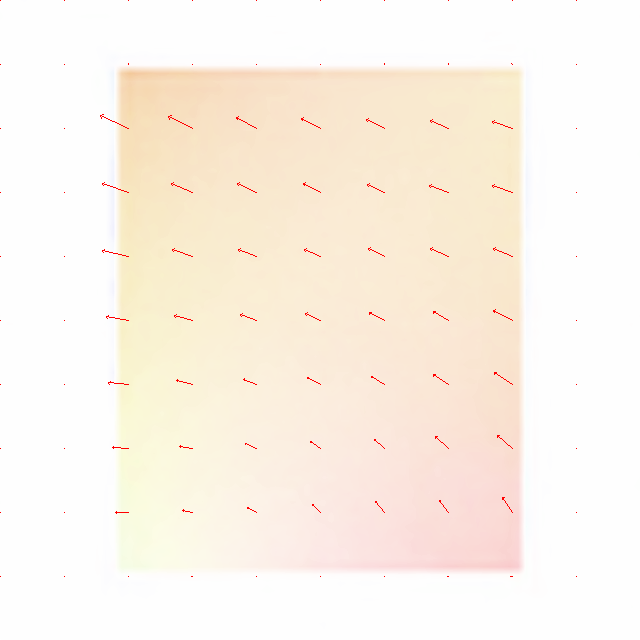
\includegraphics[width=0.12\textwidth]{Reports/4-Final-Report/images/intrinsic_metric/flow1.png}\\ 
    \end{tabular}
    \caption{The top row shows the pretrained flow model's flow output at the start of training, and the second row shows the model's flow output at the the end of training. The model shows that it has learned to be invariant to different aspect ratios.}
    \label{fig:flow_supervision}
\end{figure}





\clearpage
\subsection{Qualitative Analysis and Examples}

In figure \ref{fig:tartanvo-opticalflow}, the bottom image, illustrates the optical flow representation while executing the TartanVO baseline on KITTI Odometry Trajectory - Sequence 10. This visualization provided valuable insights that informed the design of the model's structure.


\begin{figure}[t]
    \centering
    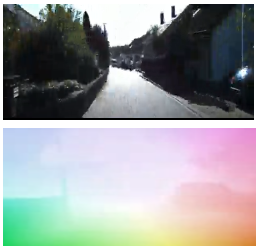
\includegraphics[width=1.0\linewidth]{Reports/2-Baselines-and-Model-Proposal/images/kitti10--inp_flow_10sec.png}
    \caption{The top image displays the model input from the left image of KITTI Odometry Trajectory 10 at 10 seconds, while the bottom image shows the corresponding optical flow output.}
    \label{fig:tartanvo-opticalflow}
\end{figure}

\clearpage
\section{Future work and Limitations (1 page)}
\textbf{Projection Issues}
One major limitation of our approach lies in the projection of 3D 360-degree LiDAR points onto a 2D image plane. This process inherently results in the loss of valuable information, as LiDAR points outside the camera's field of view are ignored. While this method provides direct correspondences between LiDAR points and image pixels, it neglects the rich spatial context of unprojected points. Future work could explore strategies to better leverage the full 3D point cloud, potentially through 3D feature learning or hybrid representations that combine 2D and 3D modalities.

\textbf{Sim-to-Real Gap}
Our reliance on synthetic training data introduces a notable sim-to-real gap. Synthetic LiDAR data assumes perfect 3D points, whereas real-world LiDAR sensors are affected by latency, noise, and skew. This distribution shift is particularly significant for LiDAR, as real-world sensors vary in type, configuration, and noise characteristics. While the flow-based intermediate representation helps mitigate the sim-to-real gap for RGB data by bounding the distribution shift, the LiDAR data remains more susceptible. Future work should focus on incorporating domain adaptation techniques or leveraging real-world LiDAR data to enhance model robustness and generalizability.

\textbf{Dynamic Objects}
Our model implicitly disregards dynamic objects in the scene, treating them as outliers or noise. While this simplifies the learning process, it introduces limitations when dynamic objects play a significant role in the scene or occlude key features. Future research could address this by explicitly modeling dynamic objects, allowing the system to adapt to their presence and even utilize their motion for additional context in odometry estimation.

\textbf{Different Datasets}
Our training and evaluation rely on a limited set of datasets, which may restrict the model's ability to generalize across different camera parameters, image shapes, and LiDAR configurations. Adding diverse datasets with varying sensor setups—such as different camera focal lengths, aspect ratios, and LiDAR types—can help the model become more robust to diverse real-world scenarios. This would enable better handling of varied intrinsic and extrinsic parameters, further reducing overfitting to specific dataset characteristics.

\textbf{LiDAR Processing}
Currently, our approach directly projects LiDAR points onto the 2D image frame for correspondences, without additional processing of the LiDAR data. This simplistic method may overlook useful spatial and structural information in the LiDAR point cloud. Future work could involve explicitly encoding LiDAR data into higher-dimensional features, such as LiDAR-specific embeddings or learned 3D features. These representations could improve the model’s understanding of spatial geometry and enhance its performance in odometry estimation. Techniques from works like point cloud learning could be explored to better utilize LiDAR data.

\textbf{Better Fusion}
Our current approach relies on cross-attention mechanisms applied to concatenated inputs of image, flow, and LiDAR data. While effective to some extent, this implicit fusion may not fully capture the complementary information between modalities. More explicit fusion techniques, such as learning shared feature spaces or designing fusion layers that integrate geometric and visual features at multiple stages, could significantly improve performance. Future work should explore tailored fusion architectures that better align and combine the strengths of each modality, leading to richer and more informative feature representations for odometry estimation.

By addressing these limitations, future iterations of the system can achieve better performance and broader applicability in real-world, dynamic, and diverse environments.

\clearpage
\section{Ethical Concerns and Considerations}
Visual-LiDAR odometry, especially in its application to autonomous vehicles, raises some ethical concerns. Intentionally, misuse of the technology for surveillance or military purposes can infringe on privacy and human rights. Unintentionally, biases in training data, such as underrepresentation of diverse environments or certain groups of people, can lead to accidents or harm in scenarios not well-represented during development. Direct ethical concerns include the potential for malfunctions causing harm to passengers or pedestrians, while indirect concerns involve societal impacts, such as job displacement in industries reliant on human drivers. Ensuring robust, equitable, and transparent development and deployment of these technologies is critical to addressing these challenges.

\clearpage
\section{Team member contributions}
\paragraph{Pujith Kachana} contributed the proposed model architecture. Wrote the dataloading and processing code, the flow prediction code, the model and training code, the visualization code, and trained the model checkpoint. Wrote the proposed model, limitations, and ethical concerns section, and contributed to writing of introduction, related works, baselines, results, and analysis sections.

\paragraph{Shashwat Chawla} contributed ...

\paragraph{Ming-Fong Li} contributed ...

\paragraph{Yatharth Ahuja} contributed ...

% Please use 
\bibliographystyle{acl_natbib}
\bibliography{references}

%\appendix



\end{document}
